\section{Histograms on the First Run~\label{sec:first_run}} 
This section exhibits histograms on the first run of 
INC with its task length increasing from 1 second to 4,096 seconds. 
The detailed description of the base data is from Table~\ref{tab:exp_notes1}.

%\section{Experiment Notes}
\paragraph{Experiment Notes:}
Table~\ref{tab:exp_notes1} provides a short description of our experimental runs, 
on which the following histograms are based.

%% done
\begin{table}[h]
\begin{center}
\begin{tabular}{|p{3cm}|p{2cm}|p{3cm}|p{4cm}|p{3cm}|} \hline
Machine & Task Length (sec) & Description & Experiment Period & Relevant \linebreak Histograms\\ \hline
{\tt sodb9} (plugged into {\em the upper left} power strip)  &  INC1$\sim$INC64 & 1000 samples, each & 2017-03-02 $\sim$ 2017-03-04 & Figs.~\ref{fig:s9_r1_et_hist1},~\ref{fig:s9_r1_et_hist2},~\ref{fig:s9_r1_pt_hist1}, and~\ref{fig:s9_r1_pt_hist2}\\ \hline
{\tt sodb9} (plugged into {\em the upper left} power strip)  &  INC128$\sim$ INC1024 & 300 samples, each & 2017-03-04 $\sim$ 2017-03-11 & 
Figs.~\ref{fig:s9_r1_et_hist3} and~\ref{fig:s9_r1_pt_hist3}\\ \hline
{\tt sodb10} (plugged into {\em the upper left} power strip)  & INC2048 & 300 samples & 2017-03-02 $\sim$ 2017-03-09 & Figs.~\ref{fig:inc2048_r1_et_hist_v5} and~\ref{fig:inc2048_r1_hist_v5}\\ \hline
{\tt sodb12} (plugged into {\em the upper left} power strip)  & INC4096 & 300 samples & 2017-02-13 $\sim$ 2017-02-27 & Figs.~\ref{fig:inc4096_r1_et_hist_v5} and~\ref{fig:inc4096_r1_hist_v5}\\ \hline
\end{tabular}
\end{center}
\vspace{-.2in}
\caption{Notes on experiment runs used for histograms\label{tab:exp_notes1}}
\end{table}

\pagebreak

\subsection{ET}

\begin{figure}[hp!]
	\centering
	\subfigure[ET frequency on INC1 on {\tt sodb9}]{
		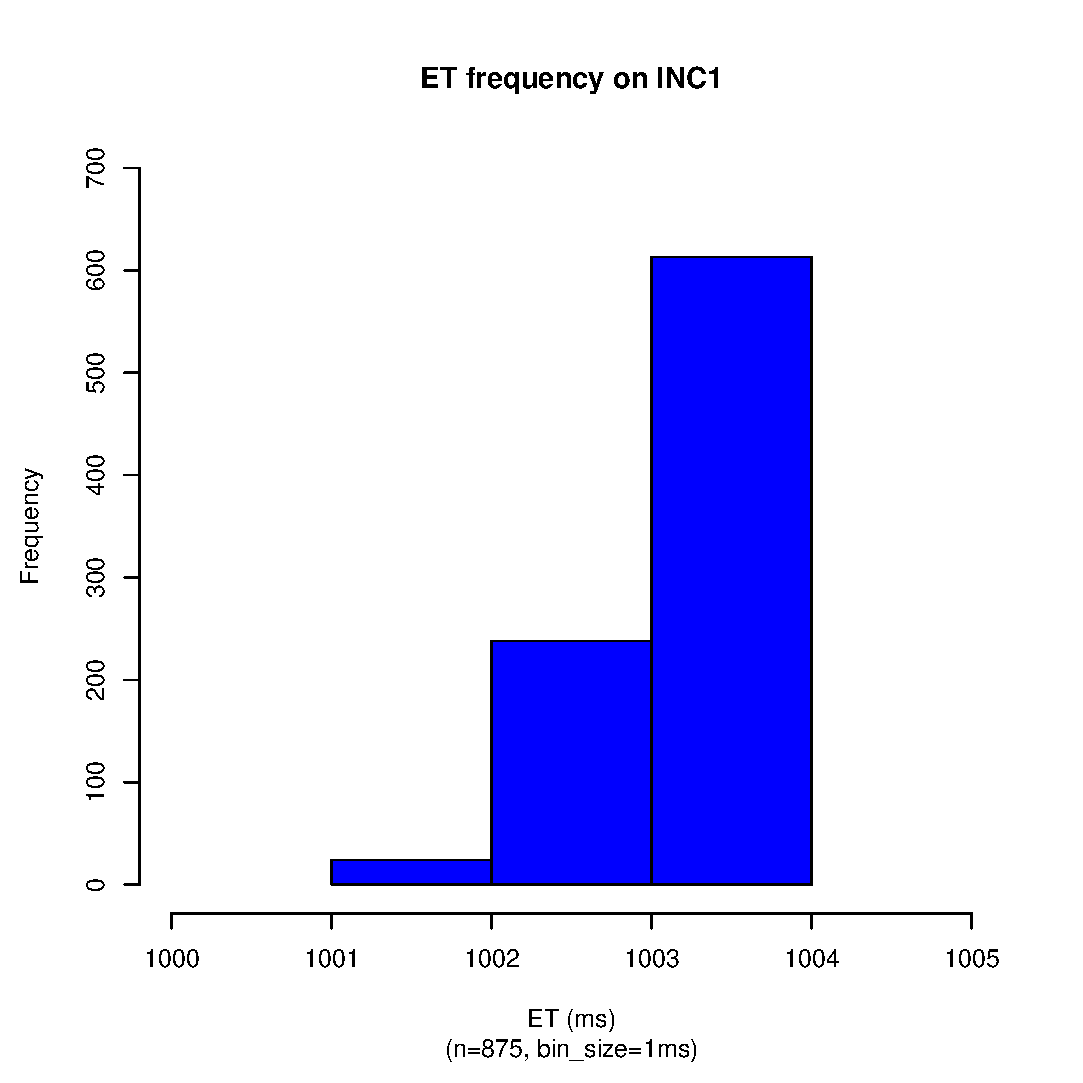
\includegraphics[scale=0.43]{repet_data1/1_sec_et_hist_v5.eps}
		\label{fig:inc1_r1_et_hist_v5}
	}
	\subfigure[ET frequency on INC2 on {\tt sodb9}]{
		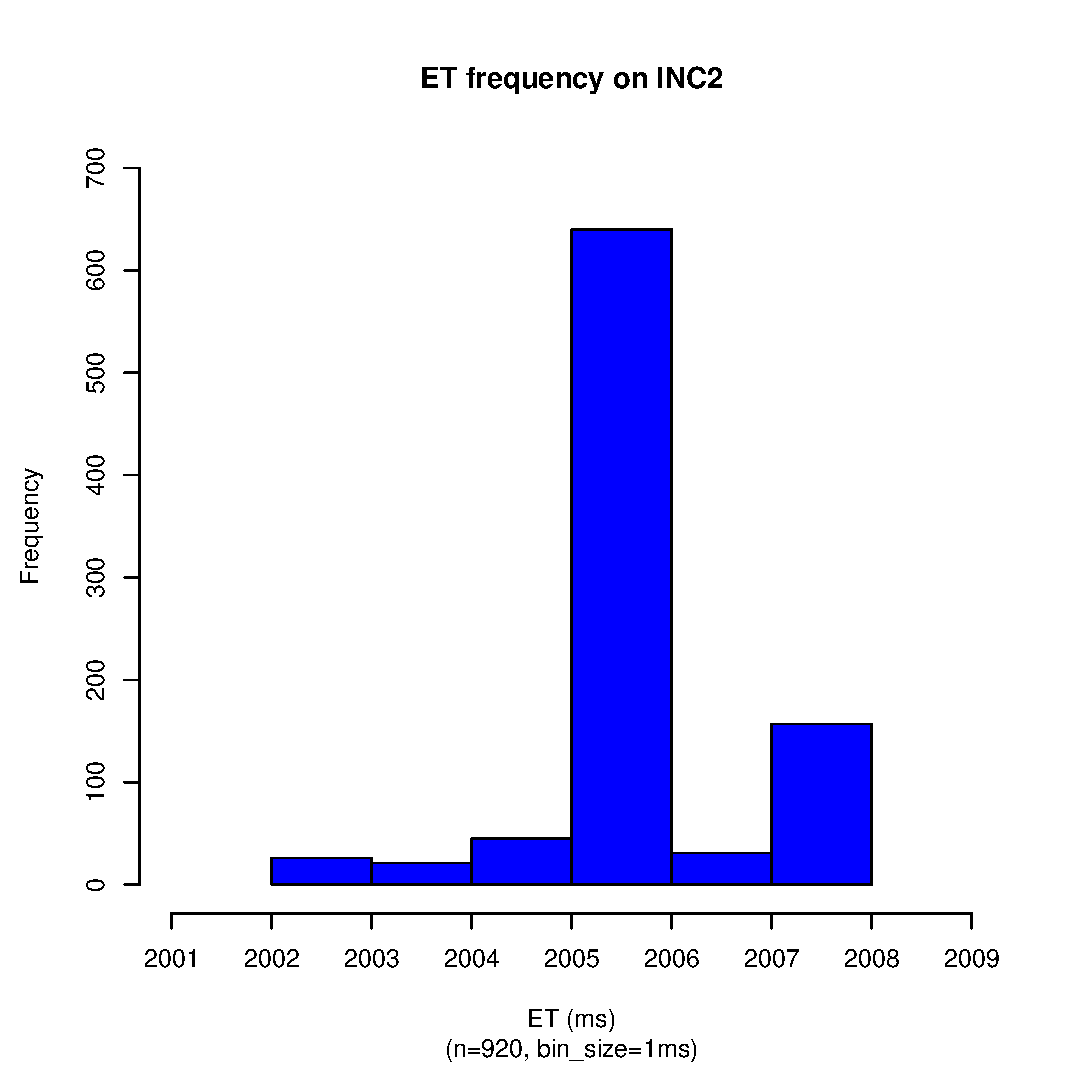
\includegraphics[scale=0.43]{repet_data1/2_sec_et_hist_v5.eps}
		\label{fig:inc2_r1_et_hist_v5}
	}
	\subfigure[ET frequency on INC4 on {\tt sodb9}]{
		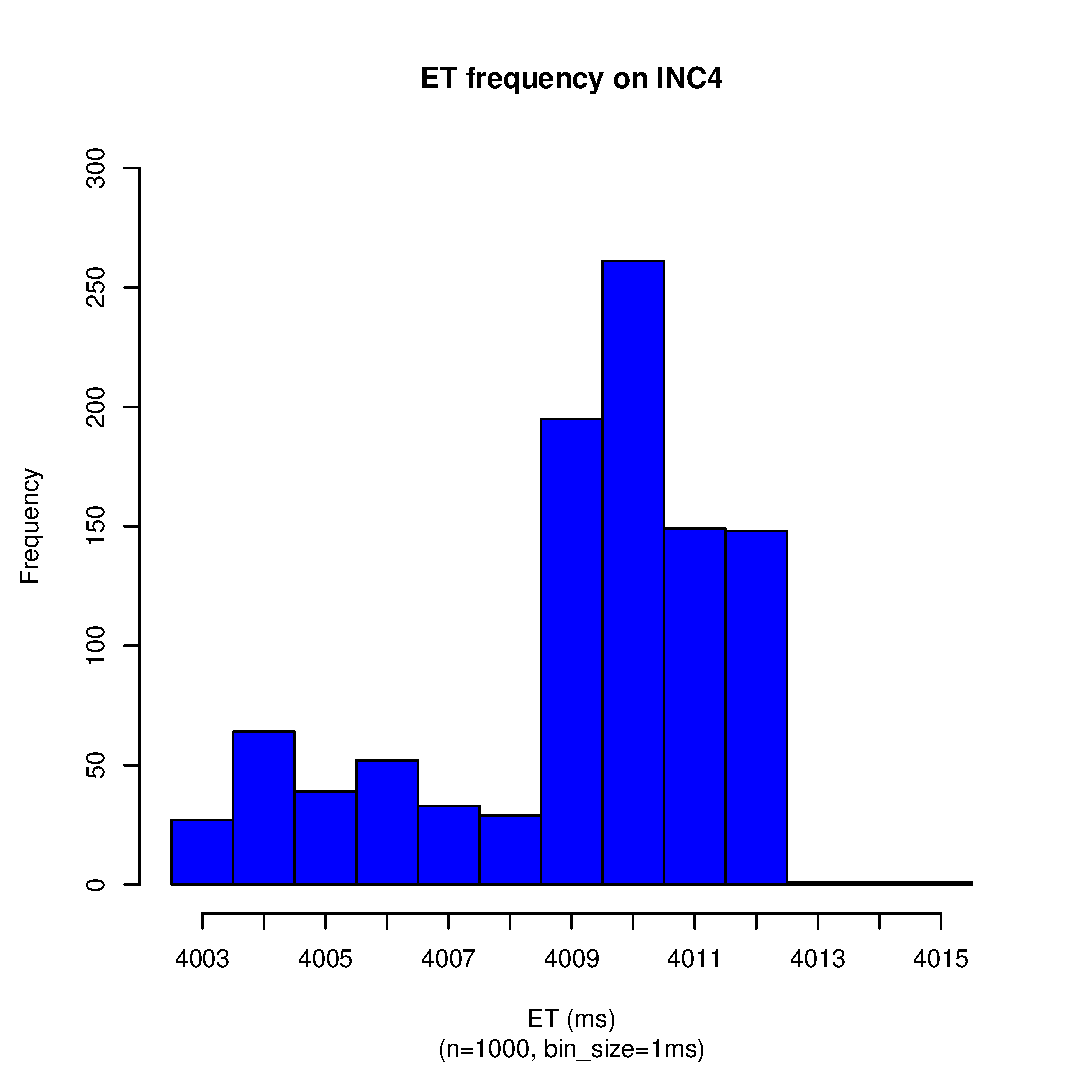
\includegraphics[scale=0.43]{repet_data1/4_sec_et_hist_v5.eps}
		\label{fig:inc4_r1_et_hist_v5}
	}
	\subfigure[ET frequency on INC8 on {\tt sodb9}]{
		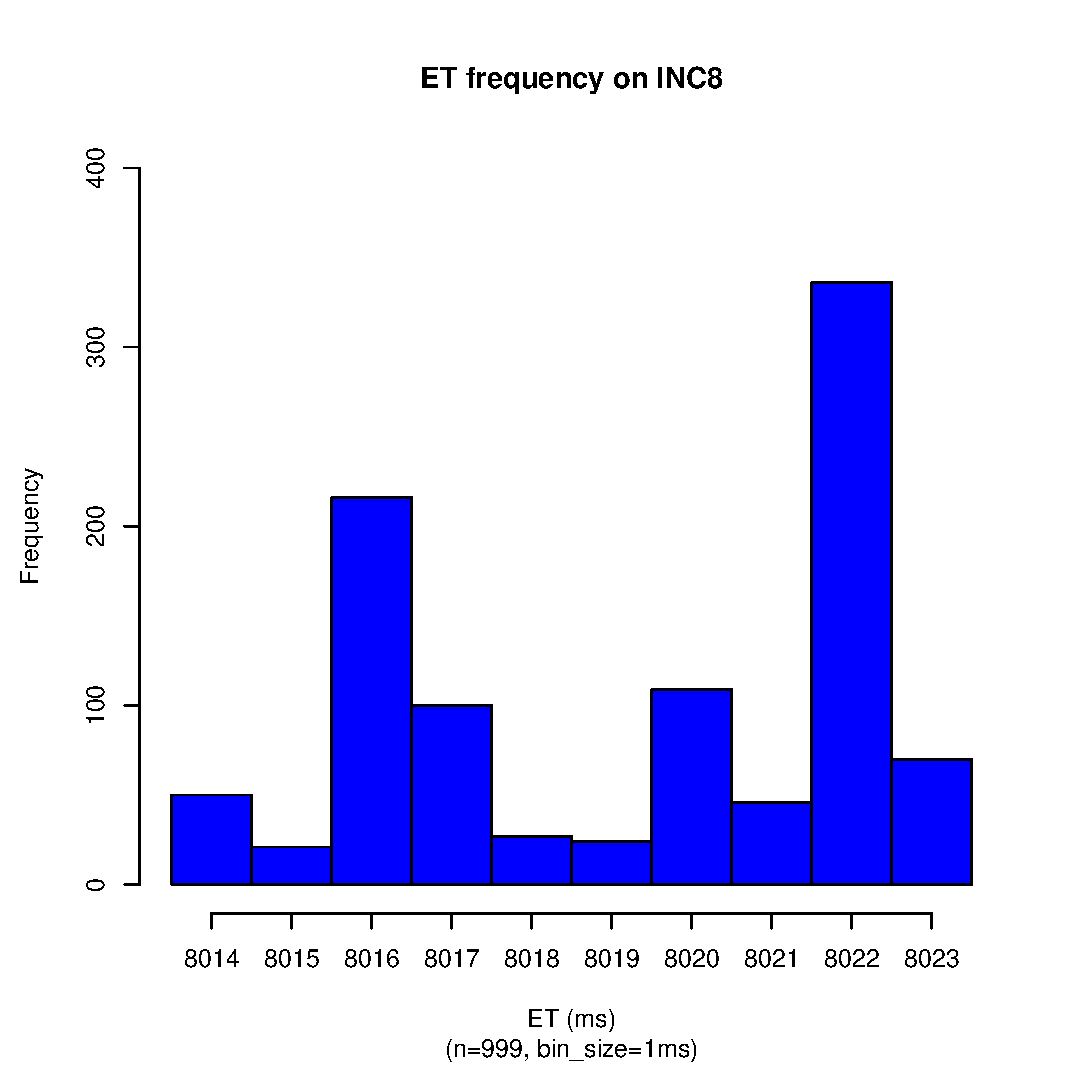
\includegraphics[scale=0.43]{repet_data1/8_sec_et_hist_v5.eps}
		\label{fig:inc8_r1_et_hist_v5}
	}
	\caption{ET Histograms of INC1 ... INC8~\label{fig:s9_r1_et_hist1}}
\end{figure}

\begin{figure}[hp!]
	\centering
	\subfigure[ET frequency on INC16 on {\tt sodb9}]{
		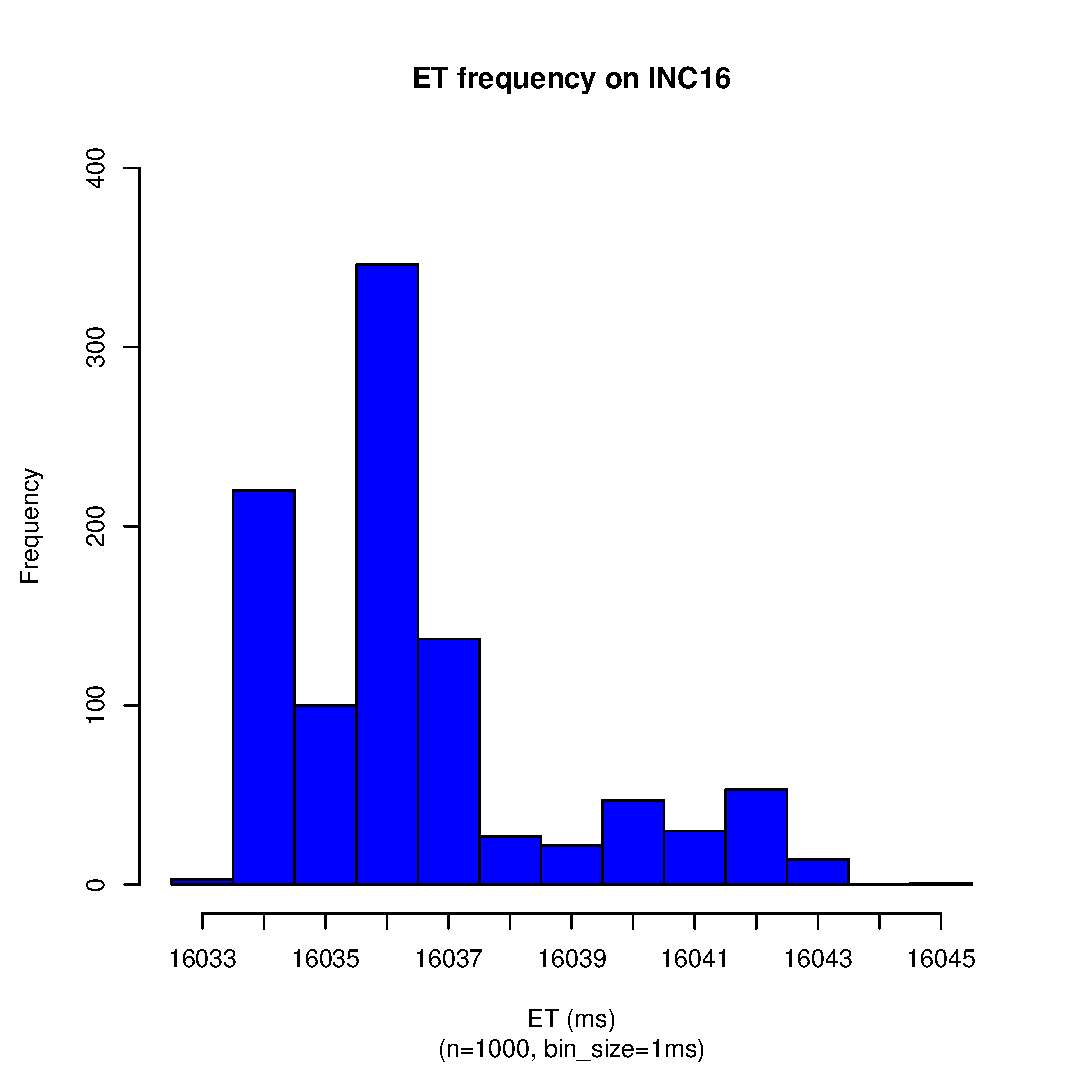
\includegraphics[scale=0.43]{repet_data1/16_sec_et_hist_v5.eps}
		\label{fig:inc16_r1_et_hist_v5}
	}
	\subfigure[ET frequency on INC32 on {\tt sodb9}]{
		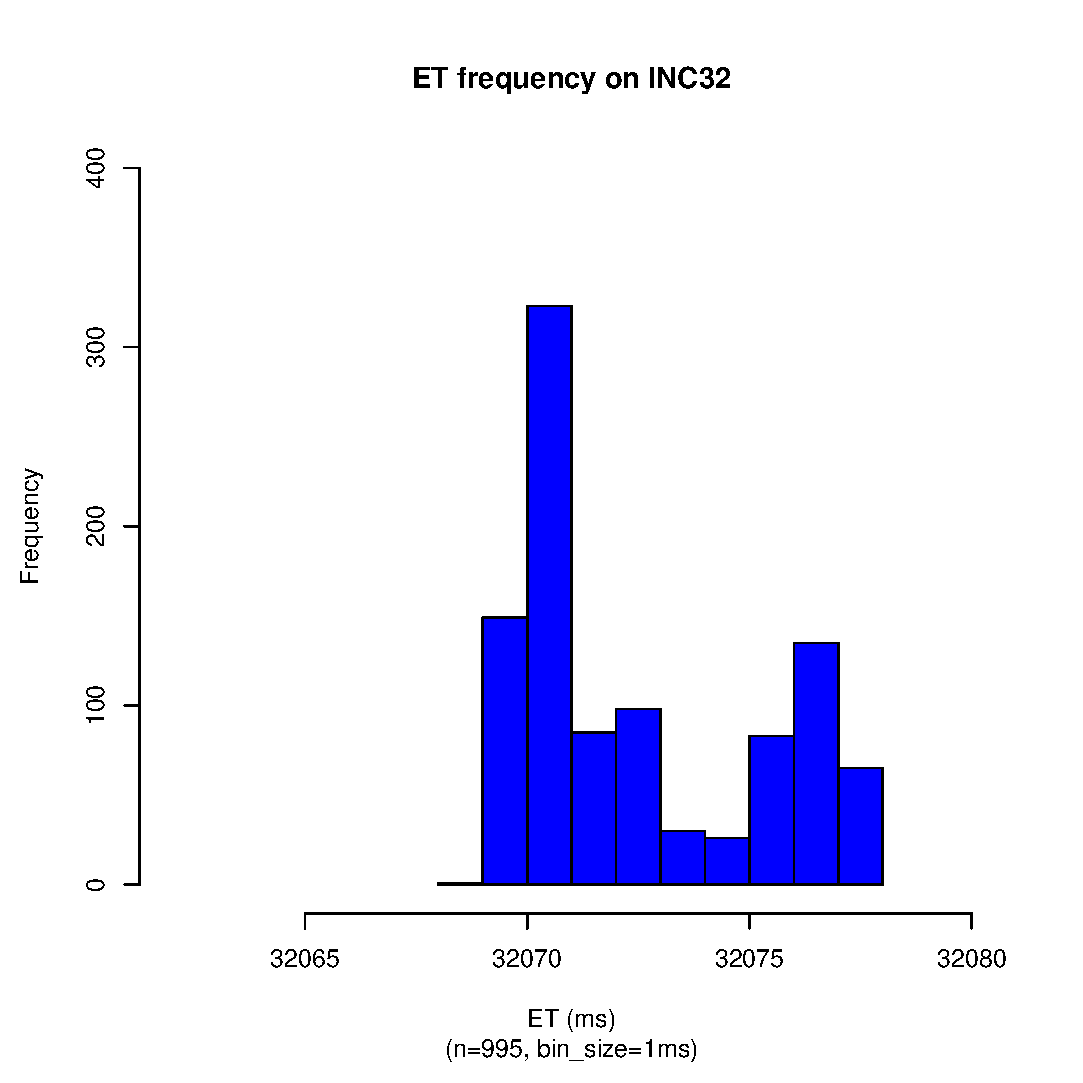
\includegraphics[scale=0.43]{repet_data1/32_sec_et_hist_v5.eps}
		\label{fig:inc32_r1_et_hist_v5}
	}
	\subfigure[ET frequency on INC64 on {\tt sodb9}]{
		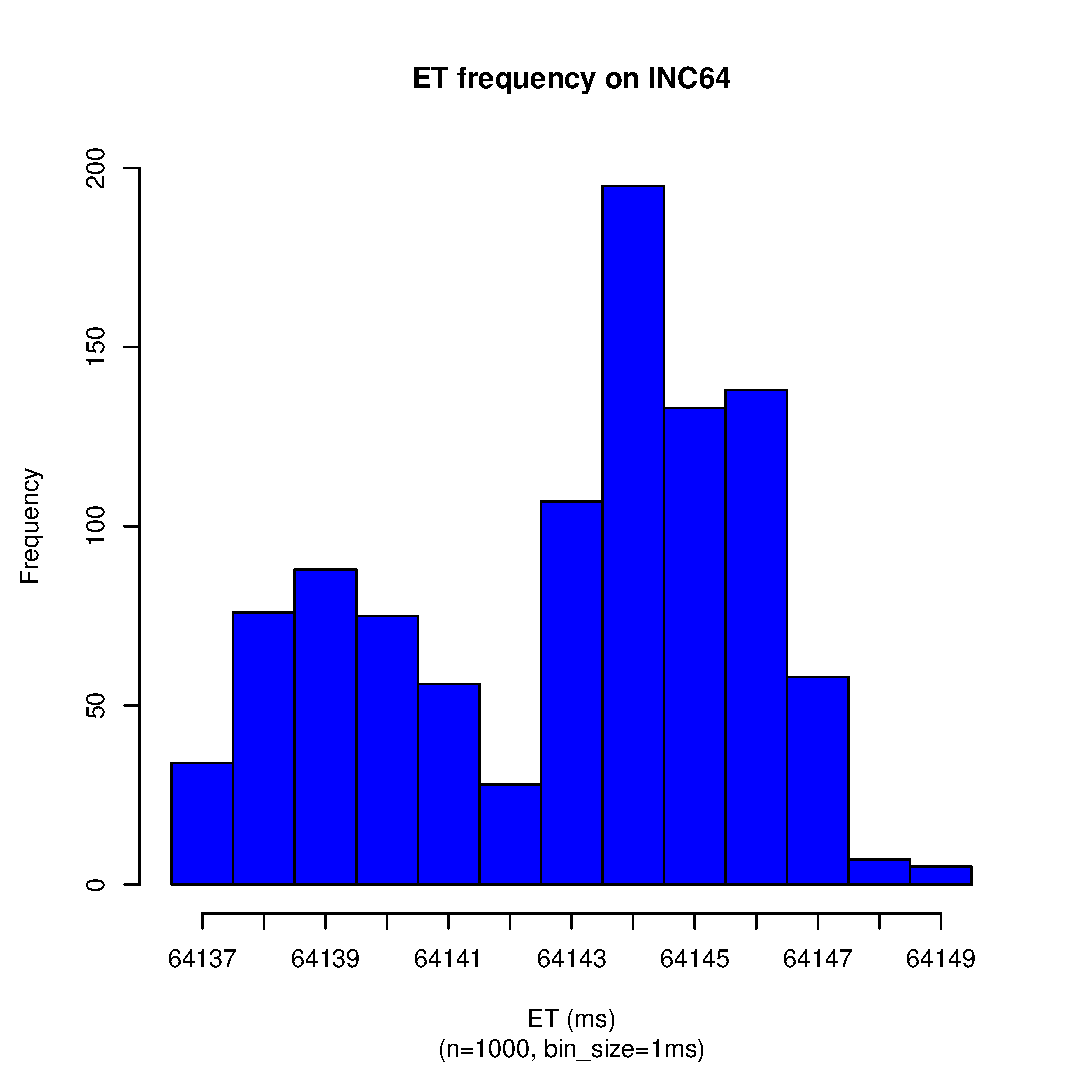
\includegraphics[scale=0.43]{repet_data1/64_sec_et_hist_v5.eps}
		\label{fig:inc64_r1_et_hist_v5}
	}
	\caption{ET Histograms of INC16 ... INC64~\label{fig:s9_r1_et_hist2}}
\end{figure}

\begin{figure}[hp!]
	\centering
	\subfigure[ET frequency on INC128 on {\tt sodb9}]{
		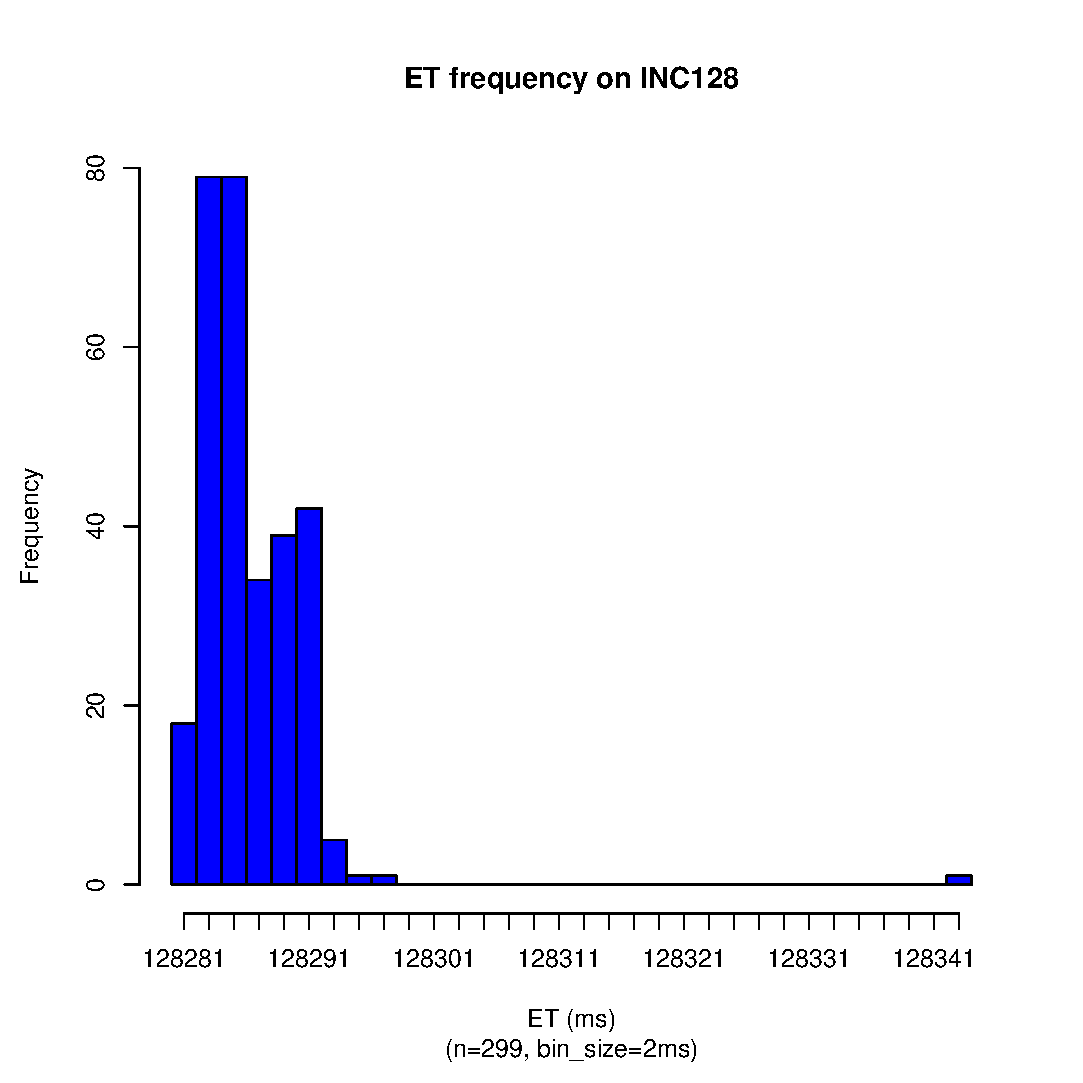
\includegraphics[scale=0.43]{repet_data1/128_sec_et_hist_v5.eps}
		\label{fig:inc128_r1_et_hist_v5}
	}
	\subfigure[ET frequency on INC256 on {\tt sodb9}]{
		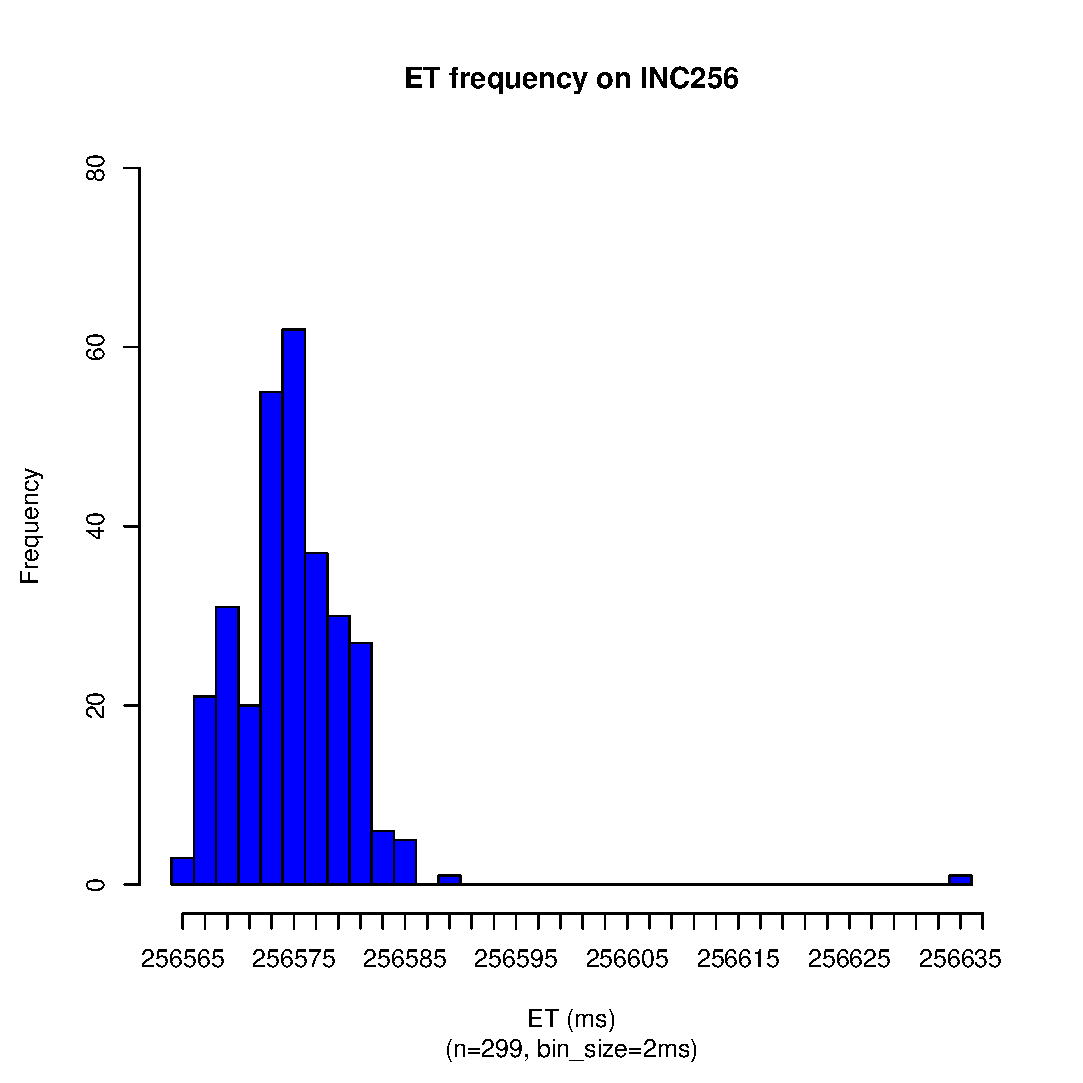
\includegraphics[scale=0.43]{repet_data1/256_sec_et_hist_v5.eps}
		\label{fig:inc256_r1_et_hist_v5}
	}
	\subfigure[ET frequency on INC512 on {\tt sodb9}]{
		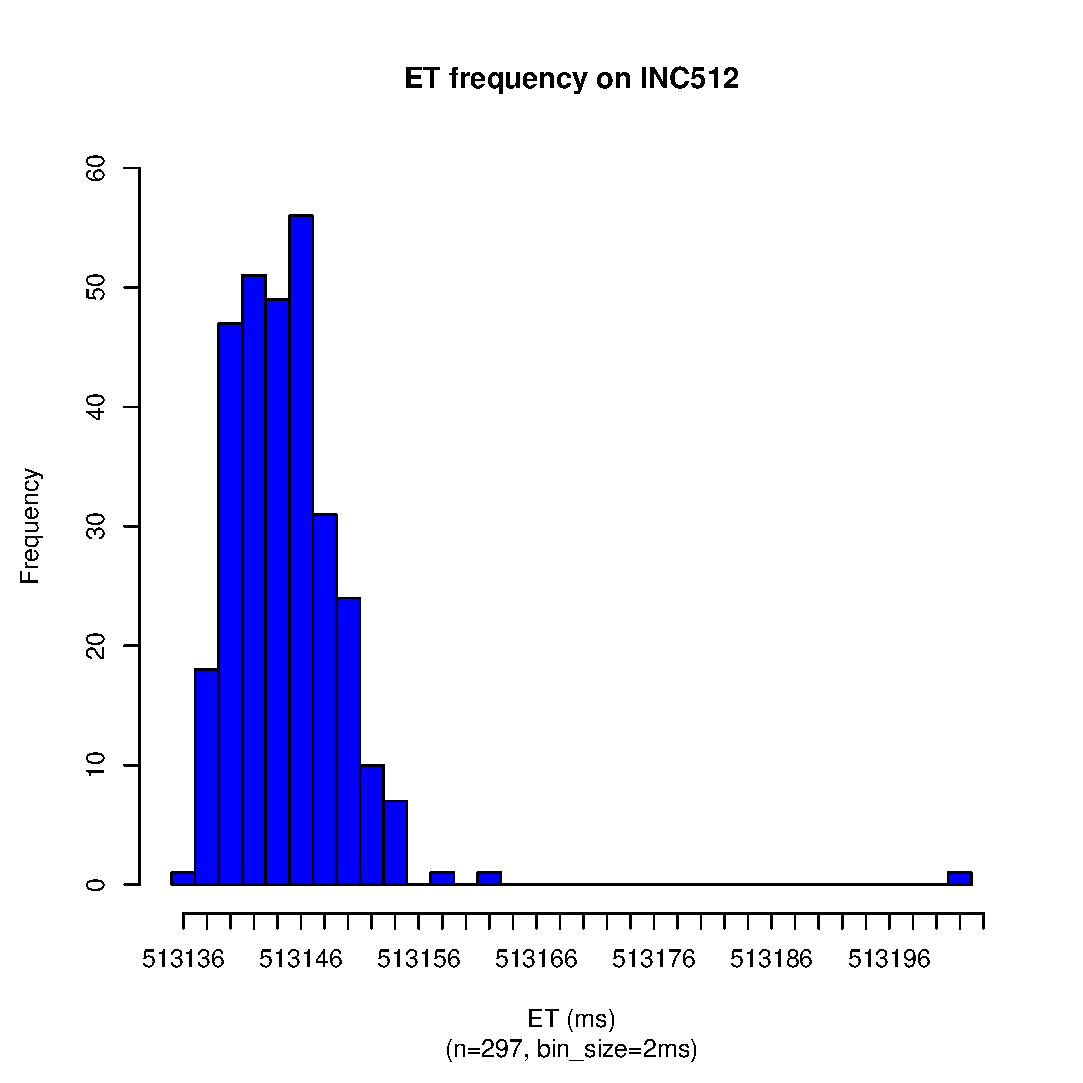
\includegraphics[scale=0.43]{repet_data1/512_sec_et_hist_v5.eps}
		\label{fig:inc512_r1_et_hist_v5}
	}
	\subfigure[ET frequency on INC1024 on {\tt sodb9}]{
		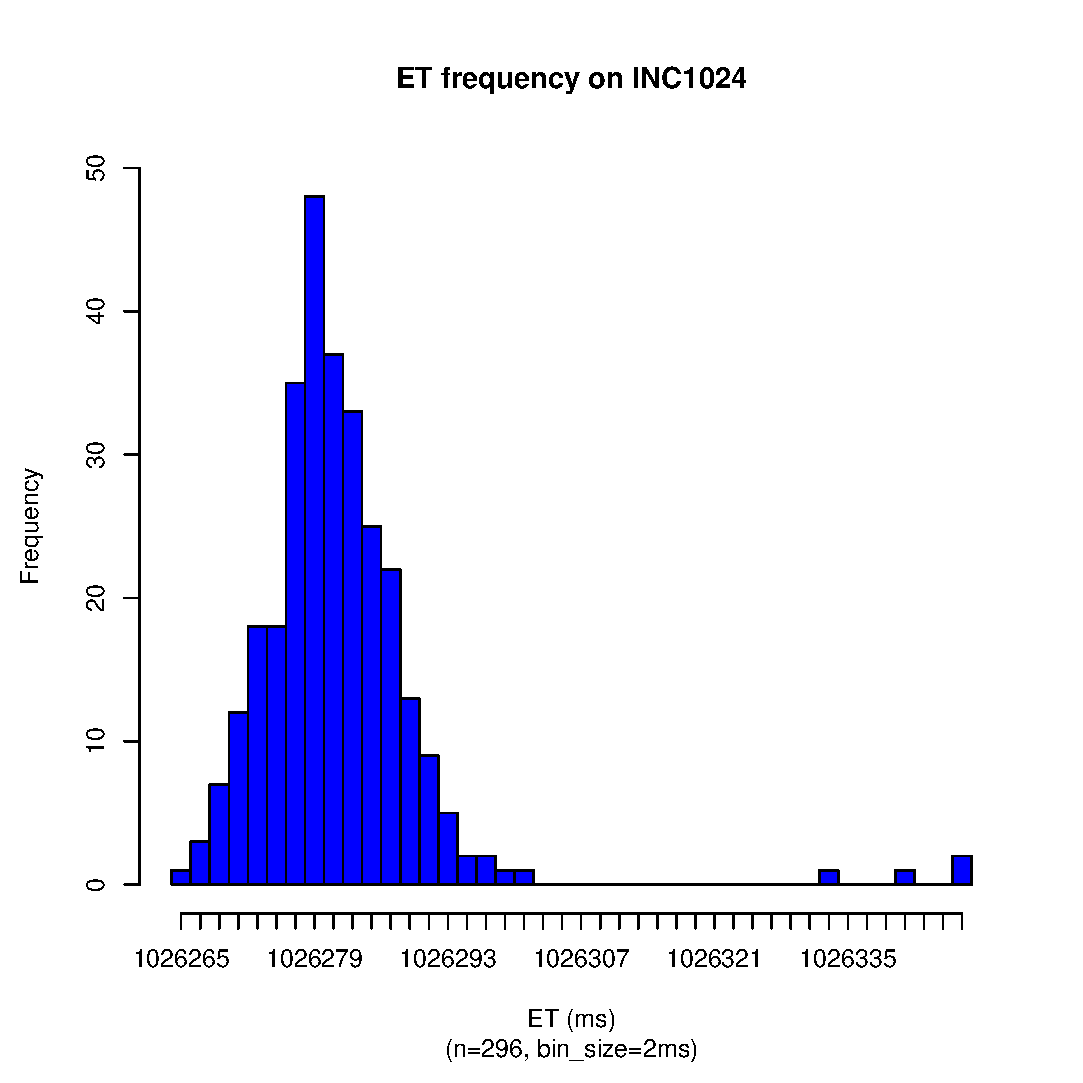
\includegraphics[scale=0.43]{repet_data1/1024_sec_et_hist_v5.eps}
		\label{fig:inc1024_r1_et_hist_v5}
	}
	\caption{ET Histograms of INC128 ... INC1024~\label{fig:s9_r1_et_hist3}}
\end{figure}

\pagebreak

\begin{figure}[t]
	\centering
	\subfigure[ET frequency on INC2048  on {\tt sodb10}]{
		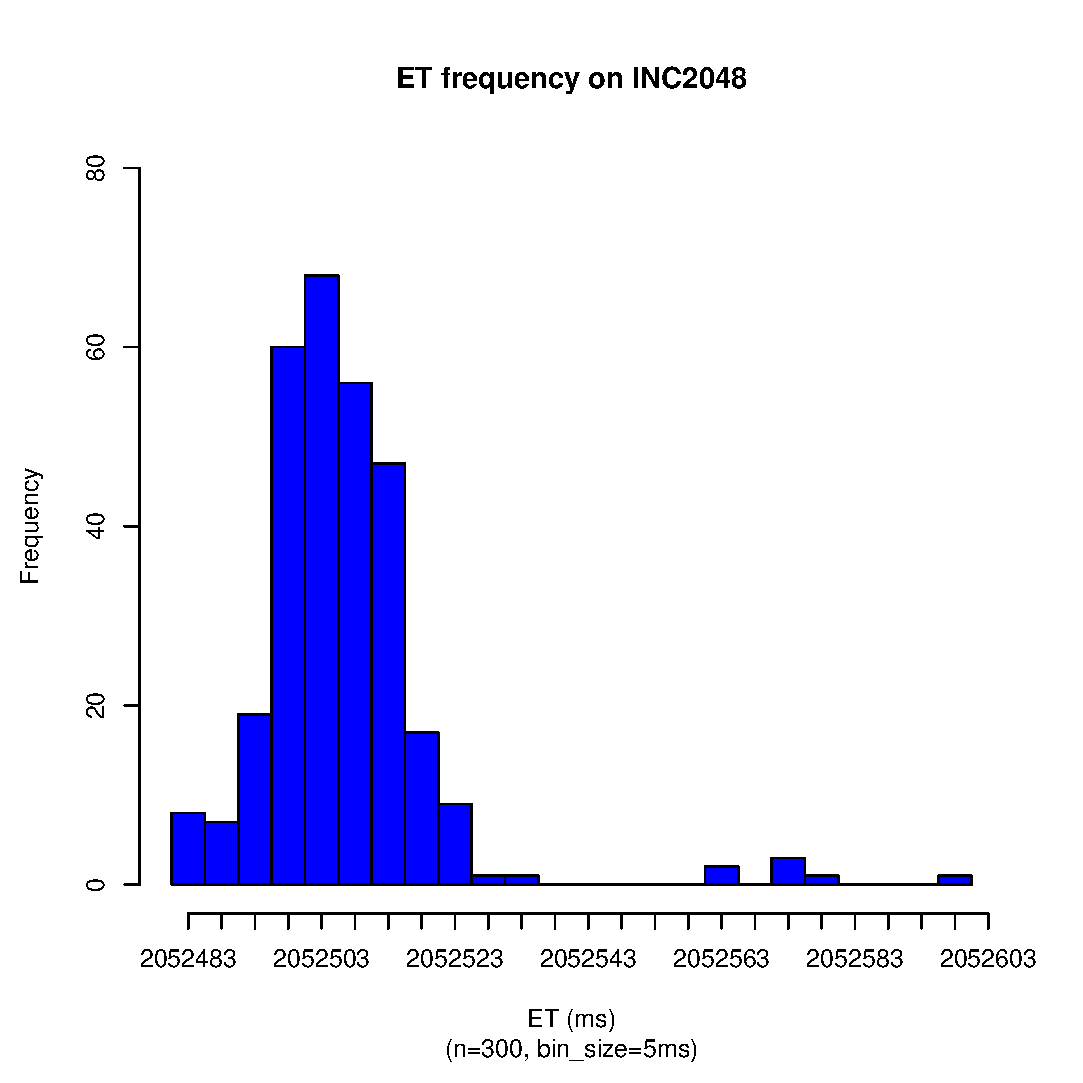
\includegraphics[scale=0.43]{repet_data1/2048_sec_et_hist_v5.eps}
		\label{fig:inc2048_r1_et_hist_v5}
	}
	\subfigure[ET frequency on INC4096 on {\tt sodb12}]{
		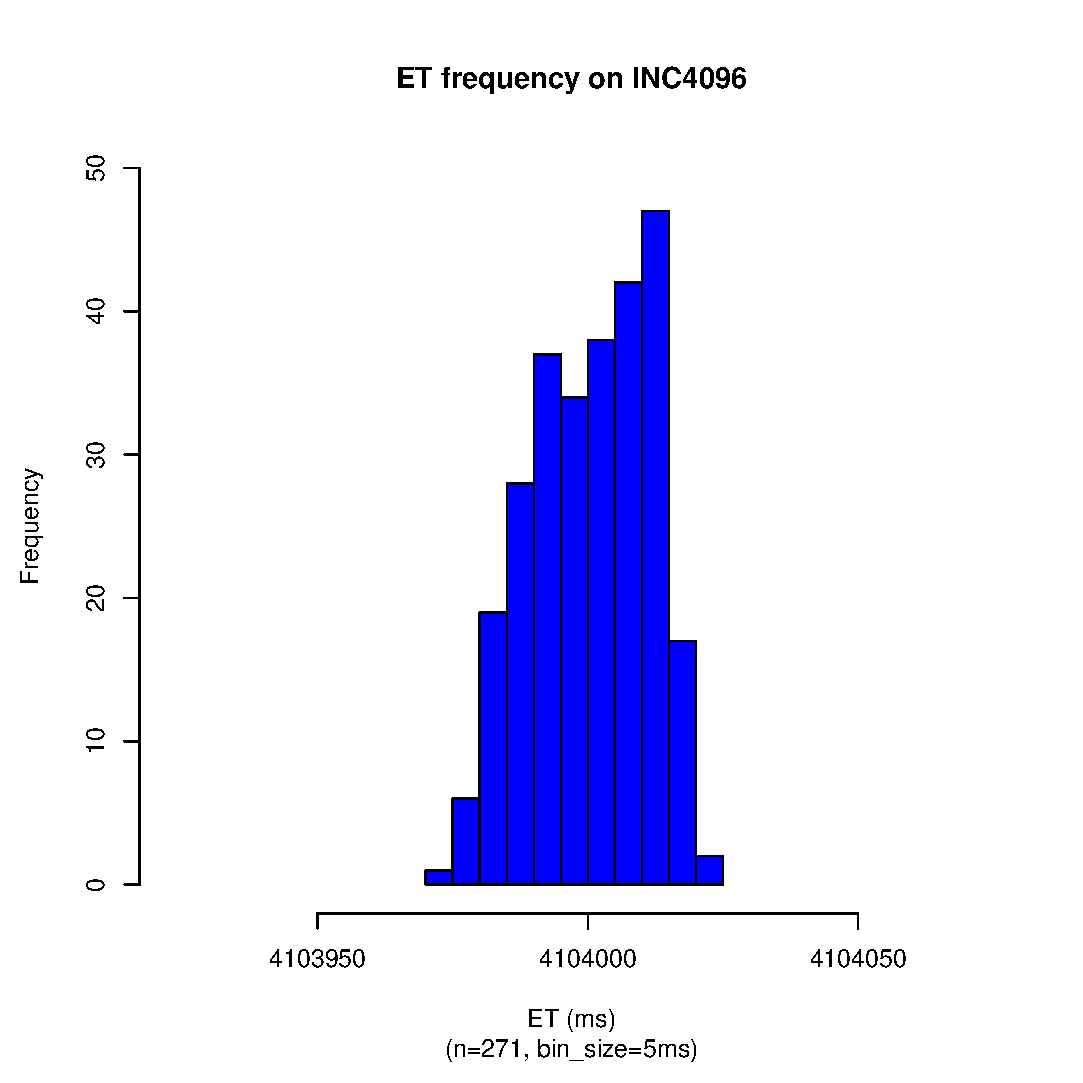
\includegraphics[scale=0.43]{repet_data1/4096_sec_et_hist_v5.eps}
		\label{fig:inc4096_r1_et_hist_v5}
	}
	\caption{ET Histograms of INC2048 and INC4096~\label{fig:s9_r1_et_hist4}}
\end{figure}

\vspace\fill
\clearpage

\subsection{PT~\label{sec:1st_pt}}

\begin{figure}[hp!]
	\centering
	\subfigure[PT frequency on INC1 on {\tt sodb9}]{
		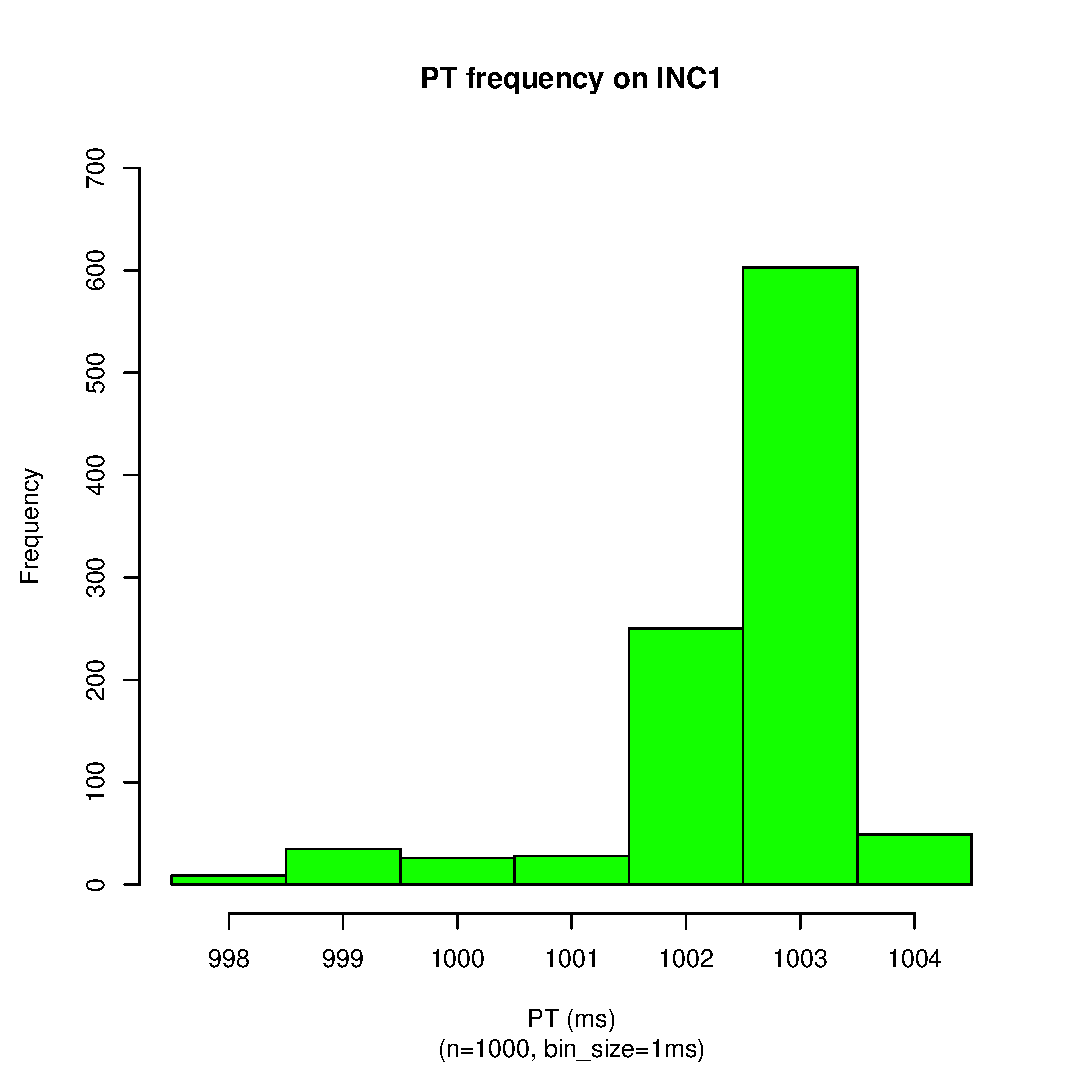
\includegraphics[scale=0.43]{repet_data1/1_sec_pt_hist_v5.eps}
		\label{fig:inc1_r1_hist_v5}
	}
	\subfigure[PT frequency on INC2 on {\tt sodb9}]{
		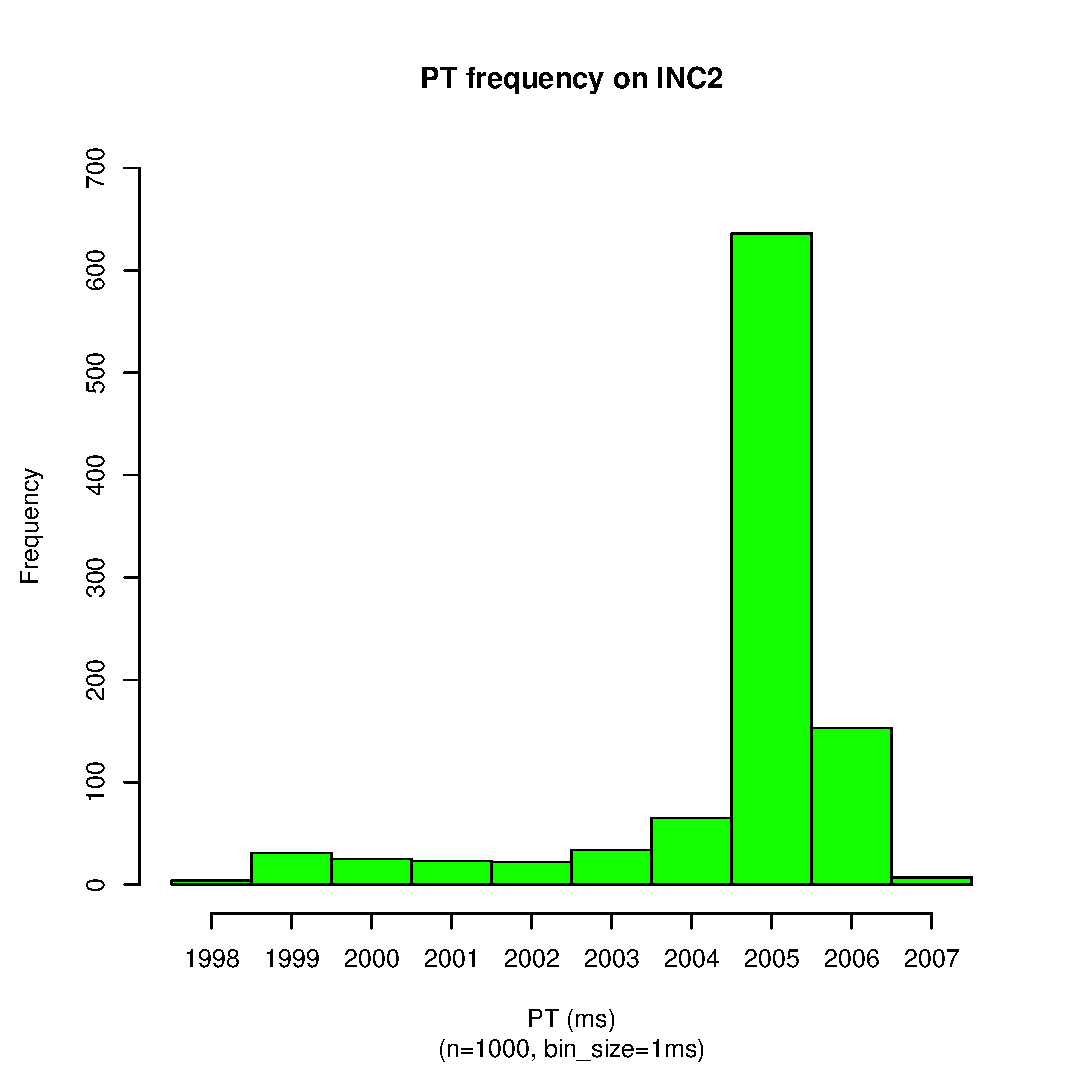
\includegraphics[scale=0.43]{repet_data1/2_sec_pt_hist_v5.eps}
		\label{fig:inc2_r1_hist_v5}
	}
	\subfigure[PT frequency on INC4 on {\tt sodb9}]{
		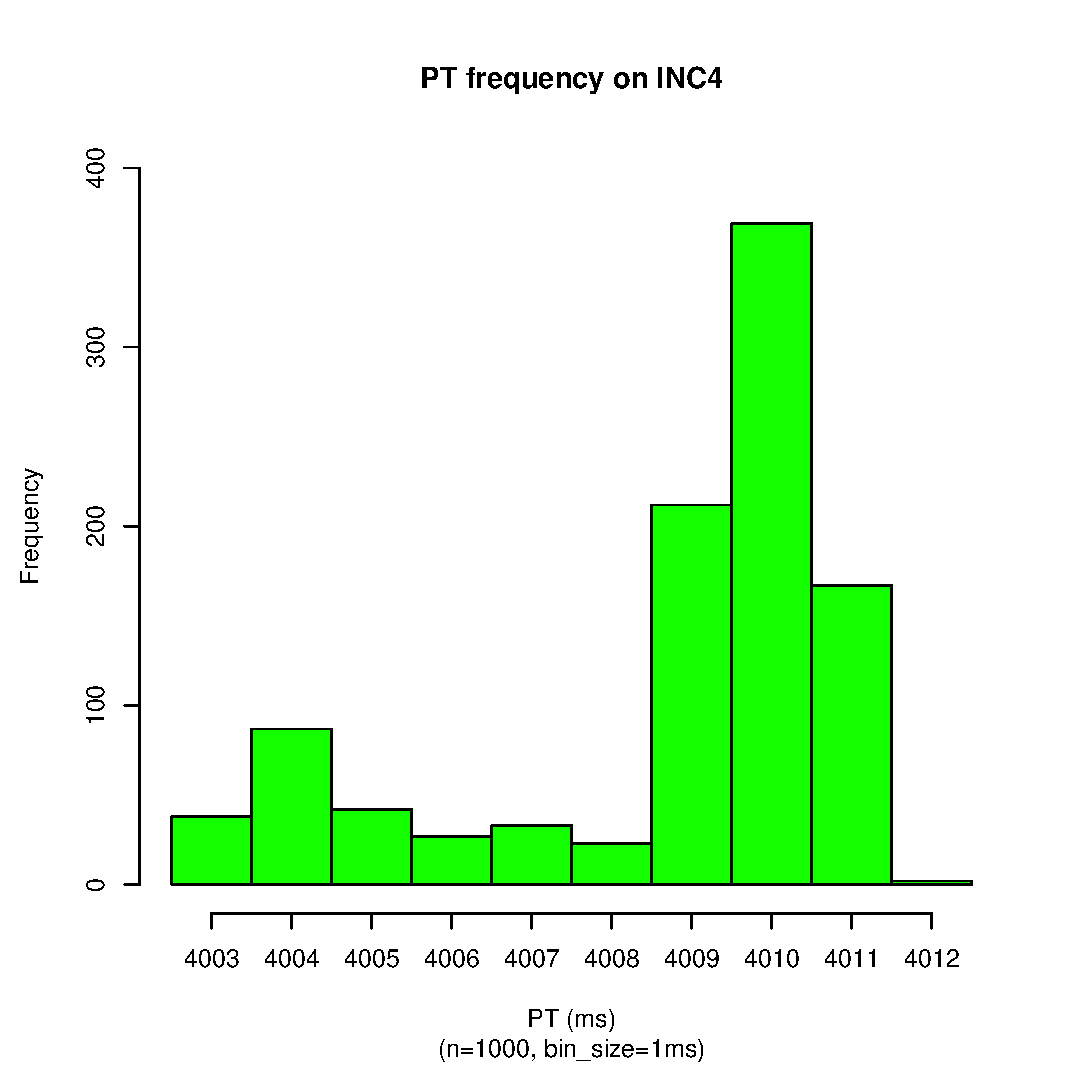
\includegraphics[scale=0.43]{repet_data1/4_sec_pt_hist_v5.eps}
		\label{fig:inc4_r1_hist_v5}
	}
	\subfigure[PT frequency on INC8 on {\tt sodb9}]{
		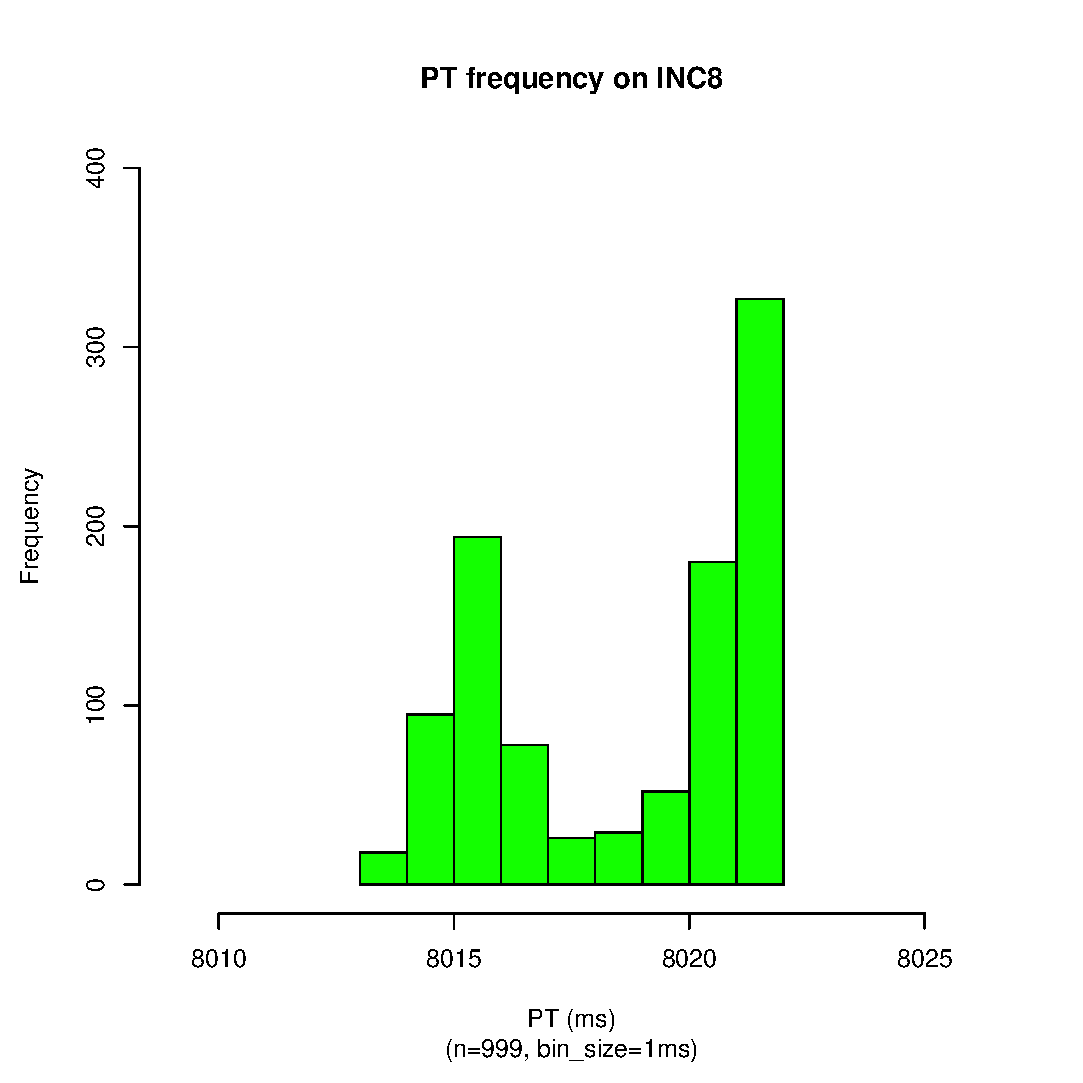
\includegraphics[scale=0.43]{repet_data1/8_sec_pt_hist_v5.eps}
		\label{fig:inc8_r1_hist_v5}
	}
	\caption{PT Histograms of INC1 ... INC8~\label{fig:s9_r1_pt_hist1}}
\end{figure}

\begin{figure}[hp!]
	\centering
	\subfigure[PT frequency on INC16 on {\tt sodb9}]{
		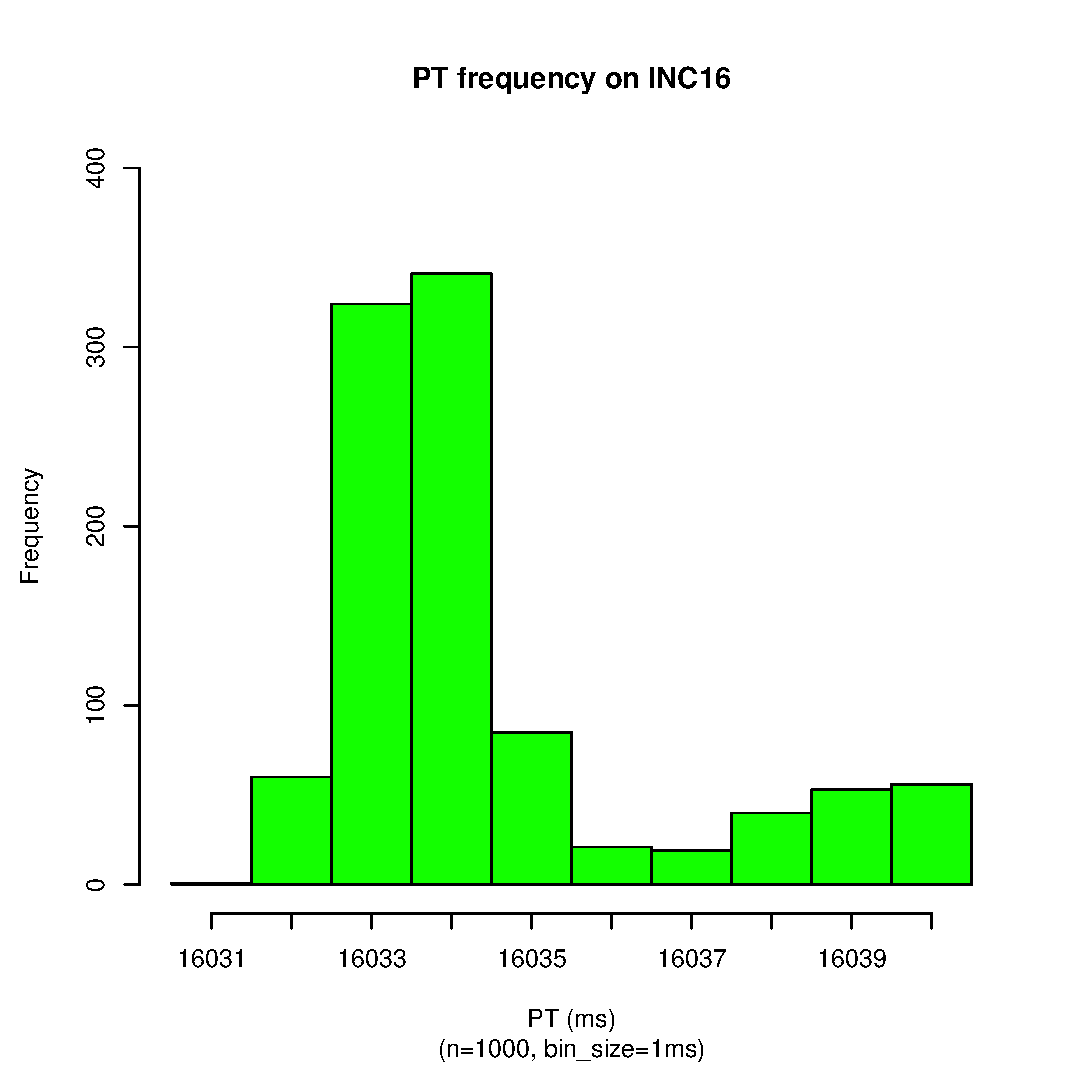
\includegraphics[scale=0.43]{repet_data1/16_sec_pt_hist_v5.eps}
		\label{fig:inc16_r1_hist_v5}
	}
	\subfigure[PT frequency on INC32 on {\tt sodb9}]{
		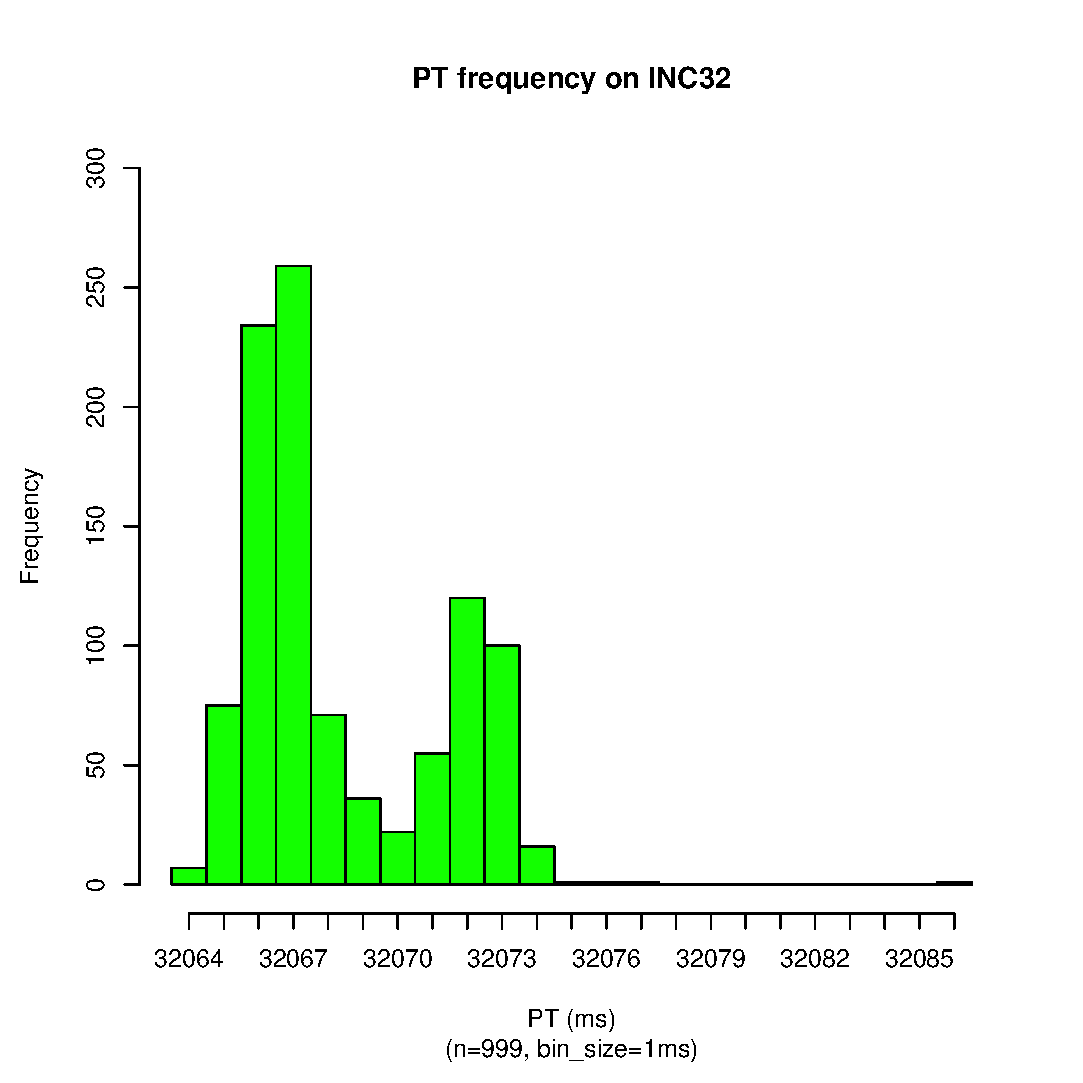
\includegraphics[scale=0.43]{repet_data1/32_sec_pt_hist_v5.eps}
		\label{fig:inc32_r1_hist_v5}
	}
	\subfigure[PT frequency on INC64 on {\tt sodb9}]{
		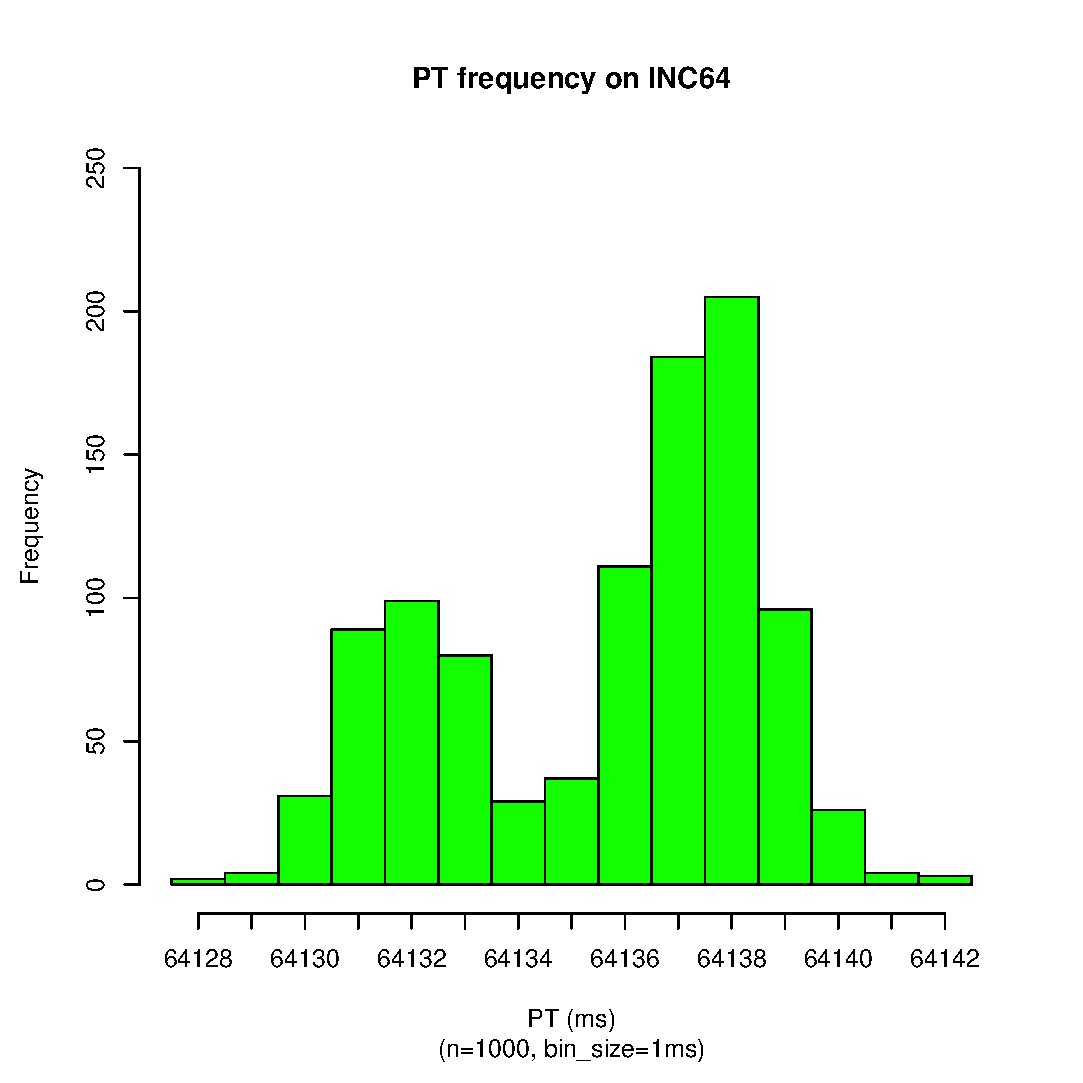
\includegraphics[scale=0.43]{repet_data1/64_sec_pt_hist_v5.eps}
		\label{fig:inc64_r1_hist_v5}
	}
	\caption{PT Histograms of INC16 ... INC64\label{fig:s9_r1_pt_hist2}}
\end{figure}

\begin{figure}[hp!]
	\centering
	\subfigure[PT frequency on INC128 on {\tt sodb9}]{
		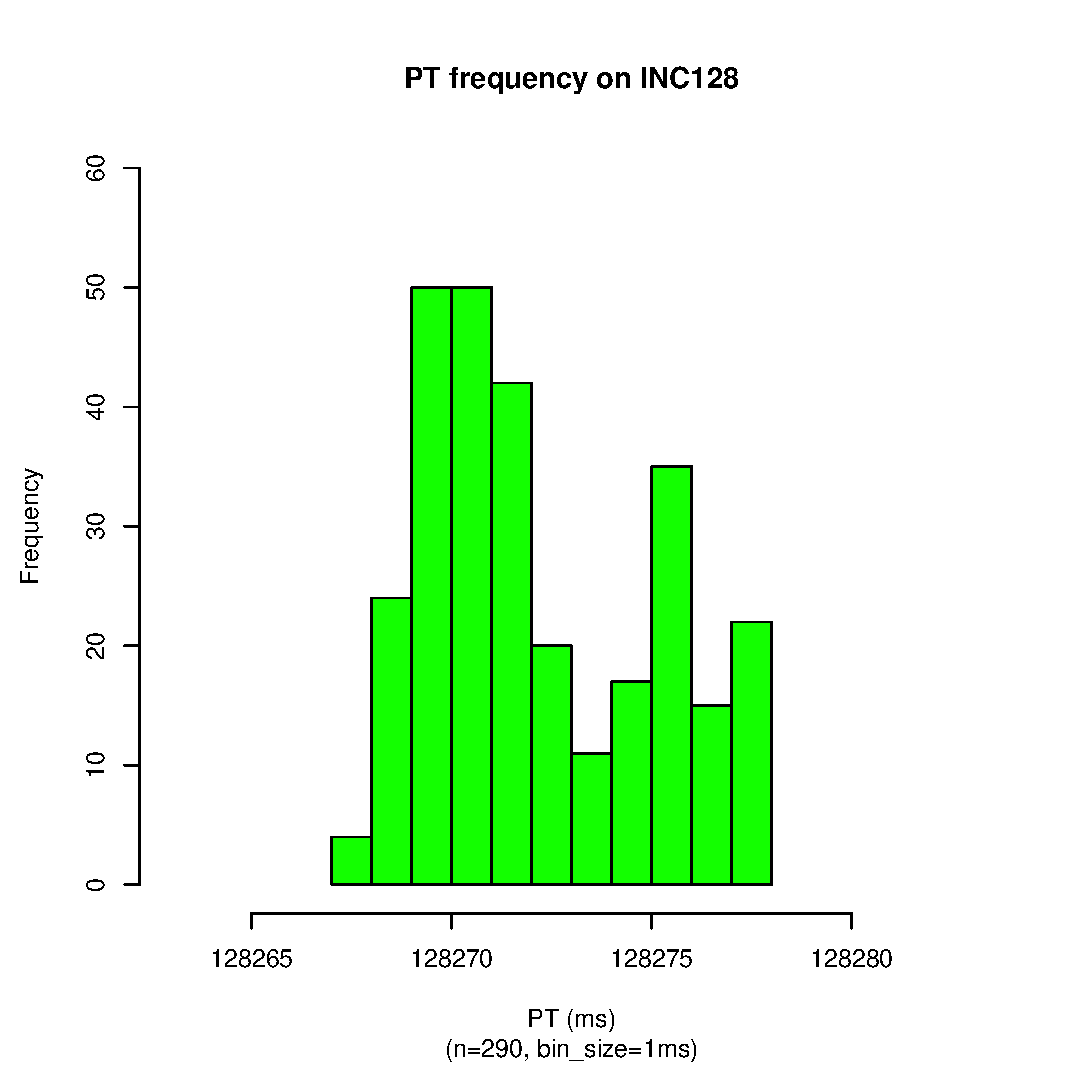
\includegraphics[scale=0.43]{repet_data1/128_sec_pt_hist_v5.eps}
		\label{fig:inc128_r1_hist_v5}
	}
	\subfigure[PT frequency on INC256 on {\tt sodb9}]{
		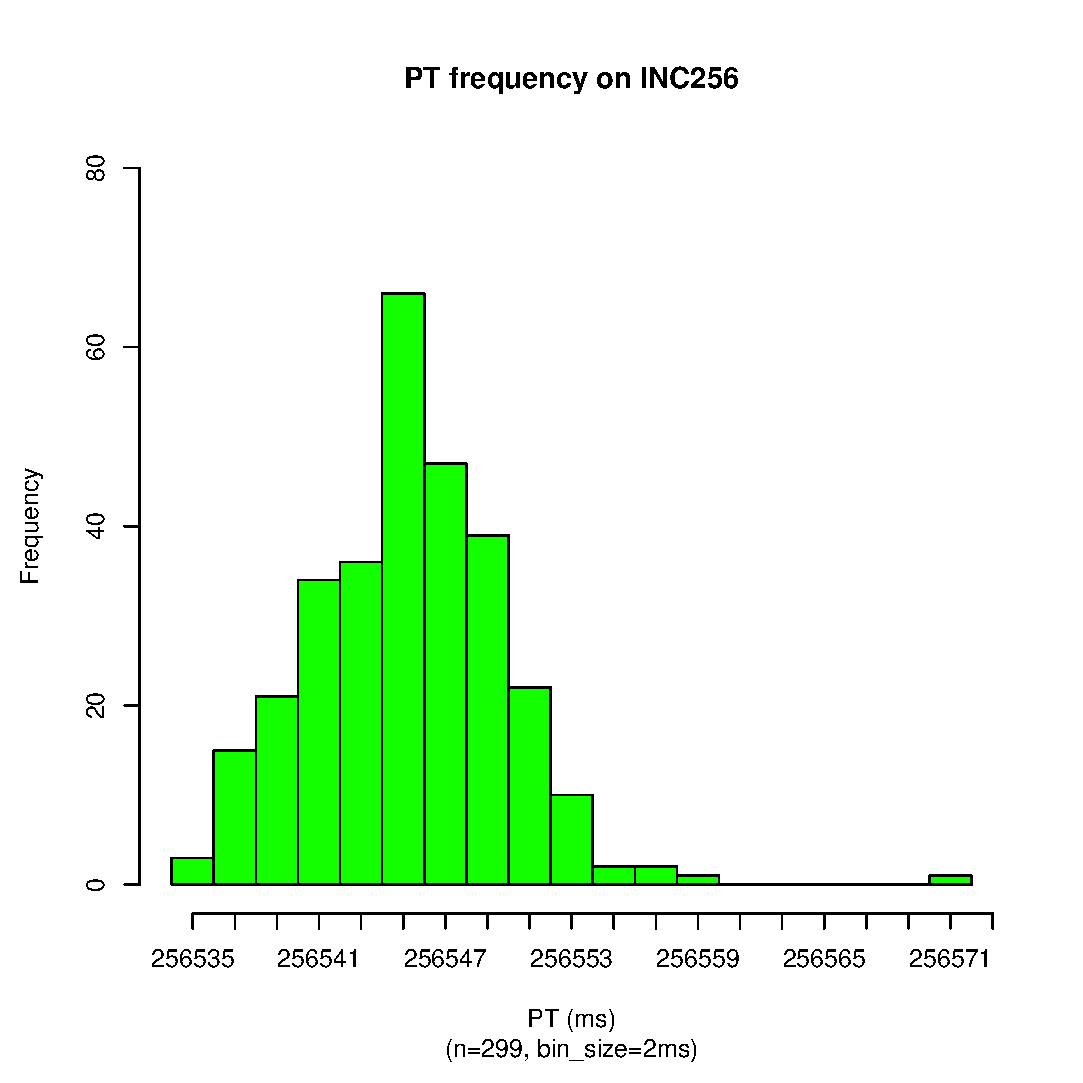
\includegraphics[scale=0.43]{repet_data1/256_sec_pt_hist_v5.eps}
		\label{fig:inc256_r1_hist_v5}
	}
	\subfigure[PT frequency on INC512 on {\tt sodb9}]{
		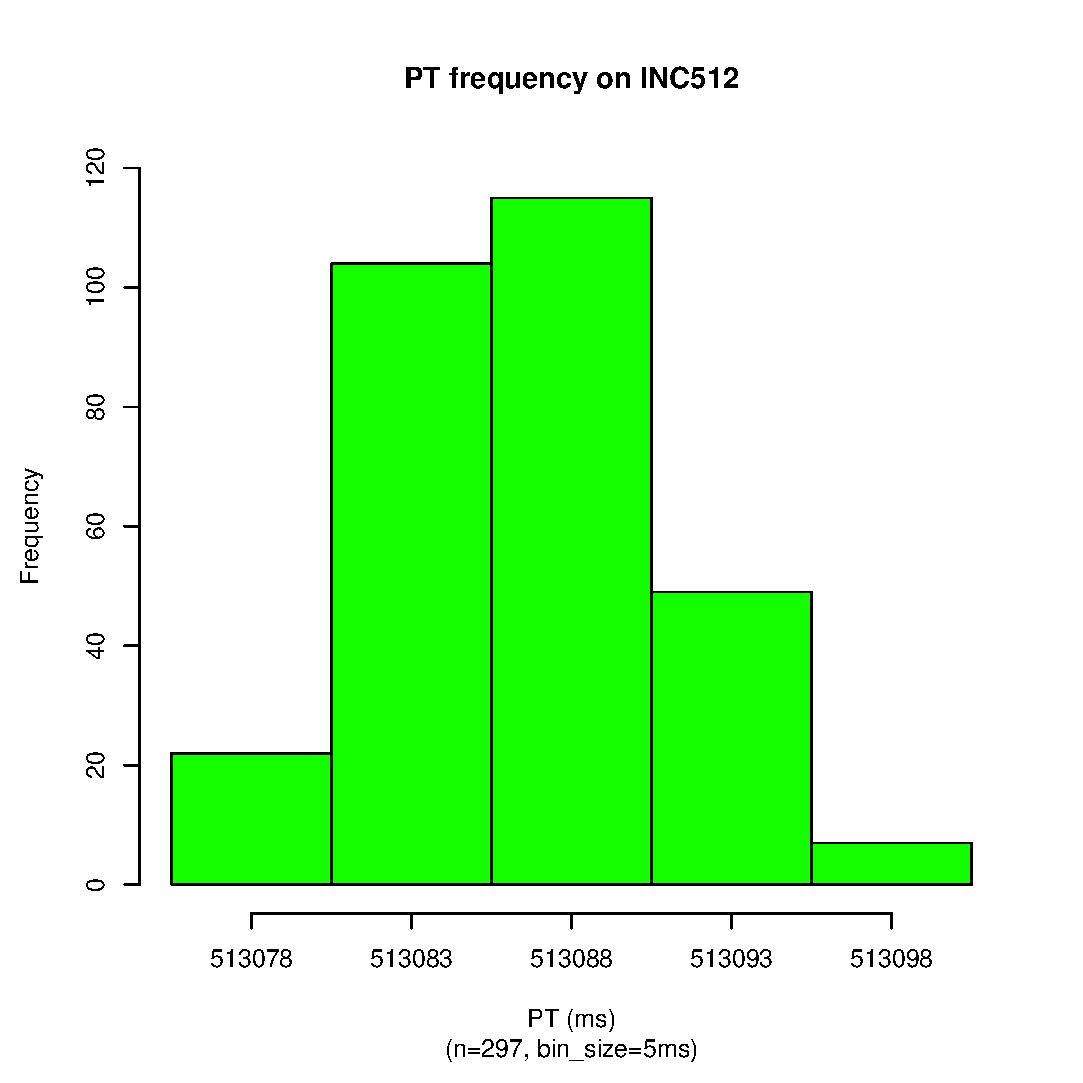
\includegraphics[scale=0.43]{repet_data1/512_sec_pt_hist_v5.eps}
		\label{fig:inc512_r1_hist_v5}
	}
	\subfigure[PT frequency on INC1024 on {\tt sodb9}]{
		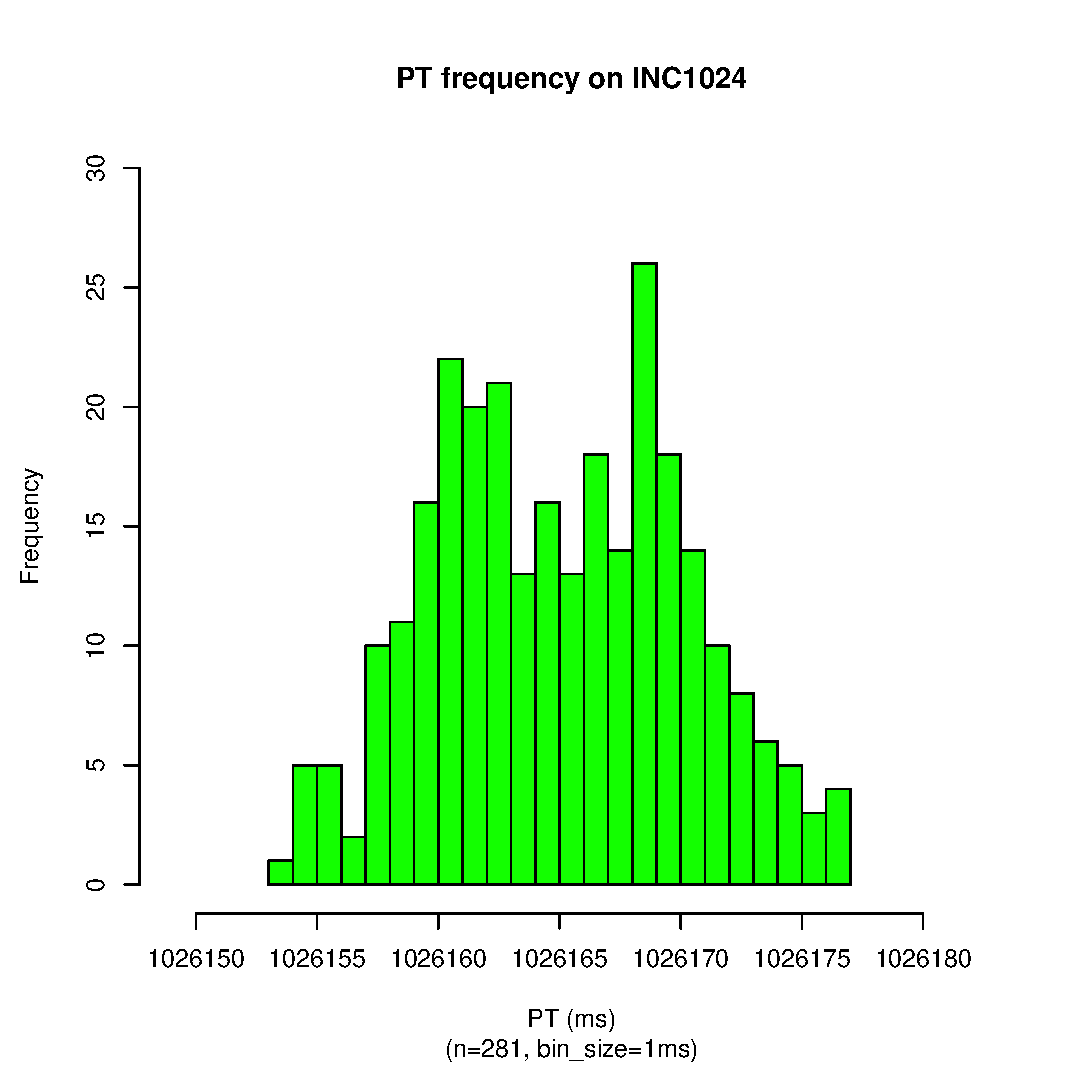
\includegraphics[scale=0.43]{repet_data1/1024_sec_pt_hist_v5.eps}
		\label{fig:inc1024_r1_hist_v5}
	}
	\caption{PT Histograms of INC256 ... INC1024~\label{fig:s9_r1_pt_hist3}}
\end{figure}

\begin{figure}[t]
	\centering
	\subfigure[PT frequency on INC2048 on {\tt sodb10}]{
		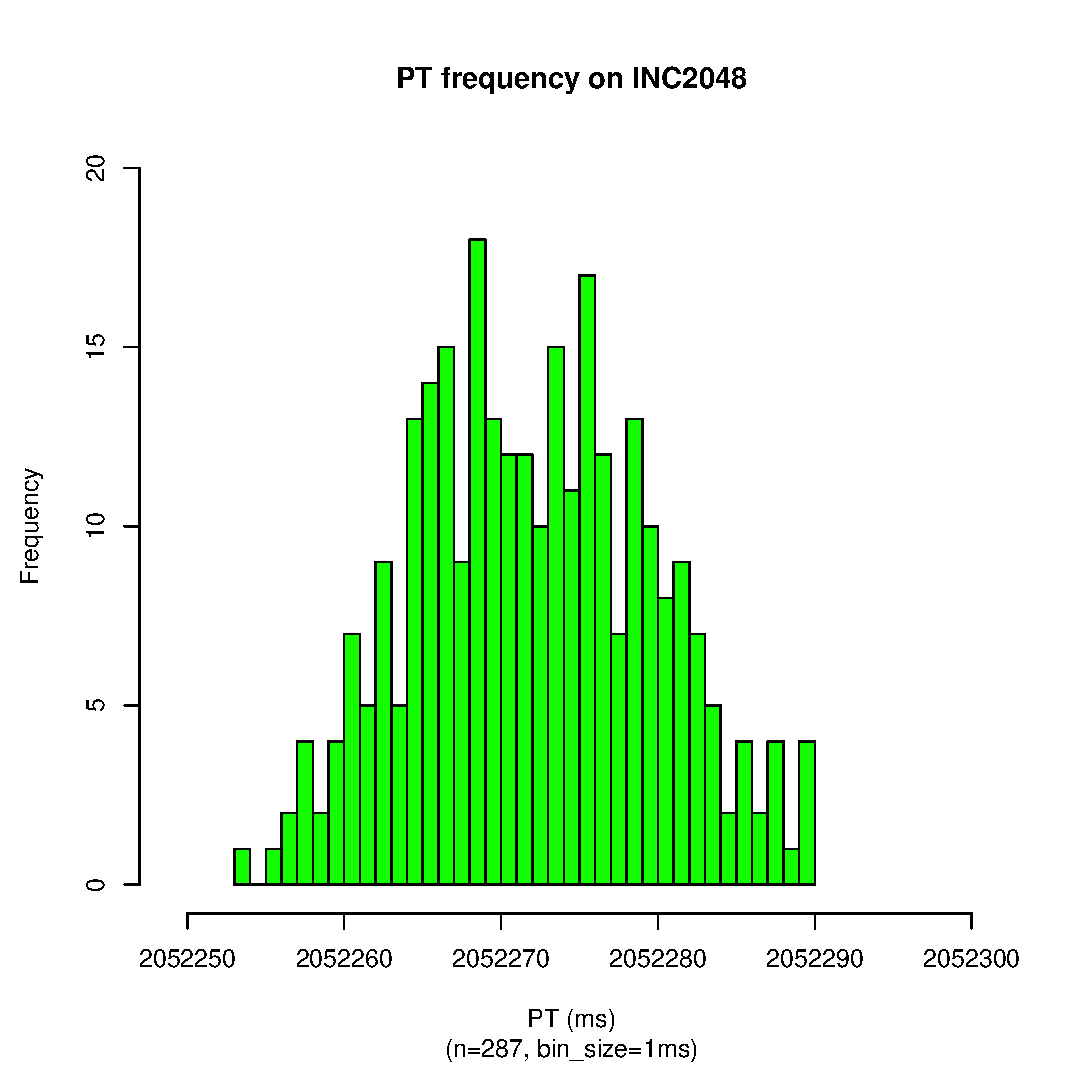
\includegraphics[scale=0.43]{repet_data1/2048_sec_pt_hist_v5.eps}
		\label{fig:inc2048_r1_hist_v5}
	}
	\subfigure[PT frequency on INC4096 on {\tt sodb12}]{
		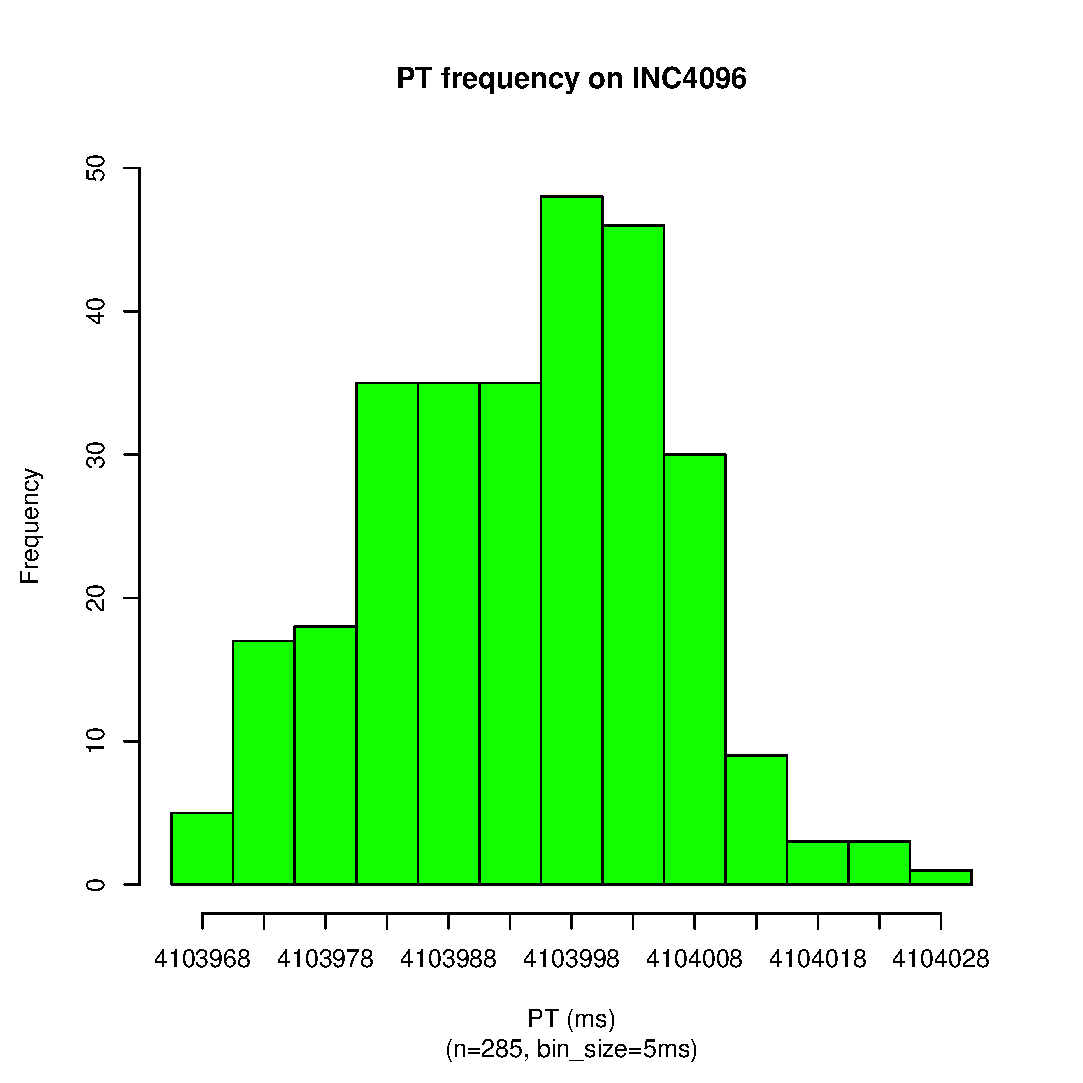
\includegraphics[scale=0.43]{repet_data1/4096_sec_pt_hist_v5.eps}
		\label{fig:inc4096_r1_hist_v5}
	}
	\caption{PT Histograms of INC2048 and INC4096~\label{fig:s9_r1_pt_hist4}}
\end{figure}

\clearpage

\pagebreak
\newpage

\subsection{Additional Histograms}
This section exhibits the histograms of INC with some intermediate task lengths under 256 secs. 
These histograms are intended to investigate where the crossing and merge of two peaks that are consistently observed up to INC128 
happened. Table~\ref{tab:exp_notes4} provides a description of the intermediate runs. 
%and the second run of INC from 8192 seconds to 16384 seconds via EMPv5 with no Step 2.
\begin{table}[h]
\begin{center}
\begin{tabular}{|p{2cm}|p{3cm}|p{3cm}|p{4cm}|p{3.5cm}|} \hline
Machine & Task Length (sec) & Description & Experiment Period & Relevant \linebreak Histograms\\ \hline
{\tt sodb9} &  INC96$\sim$INC256 & 1000 samples, each & 2017-05-24 $\sim$ 2017-06-06 & Figs.~\ref{fig:ut_hist3}, \ref{fig:inc224_ut_hist}, and~\ref{fig:inc256_ut_hist}\\ \cline{2-4}
(plugged into {\em the upper left} power strip)	&  INC3, 6, 12, 24, 48, 72, 80, 88, 104, 112, and 120 & 1000 samples, each & 2017-06-07 $\sim$ 2017-06-16 & Figs.~\ref{fig:inc3_ut_hist}, ~\ref{fig:inc6_ut_hist}, ~\ref{fig:inc12_ut_hist}, ~\ref{fig:inc24_ut_hist},
~\ref{fig:inc48_ut_hist}, ~\ref{fig:inc72_ut_hist}, ~\ref{fig:inc80_ut_hist}, ~\ref{fig:inc88_ut_hist}, ~\ref{fig:inc104_ut_hist},~\ref{fig:inc112_ut_hist}, and~\ref{fig:inc120_ut_hist}\\ \hline
\end{tabular}
\end{center}
\vspace{-.2in}
\caption{Notes on experiment runs used for histograms\label{tab:exp_notes4}}
\end{table}

\subsubsection{ET}
Not available at this point, due to the labshelf server's unavailability for the time being.

\pagebreak

\subsubsection{PT}
%The histograms of INC1 through INC4096 are 
%the same as those of Figures~\ref{fig:s9_r1_pt_hist1},~\ref{fig:s9_r1_pt_hist2},~\ref{fig:s9_r1_pt_hist3}, and~\ref{fig:s9_r1_pt_hist4}. 

\begin{figure}[hp!]
	\centering
	\subfigure[PT frequency on INC3  on {\tt sodb9}]{
		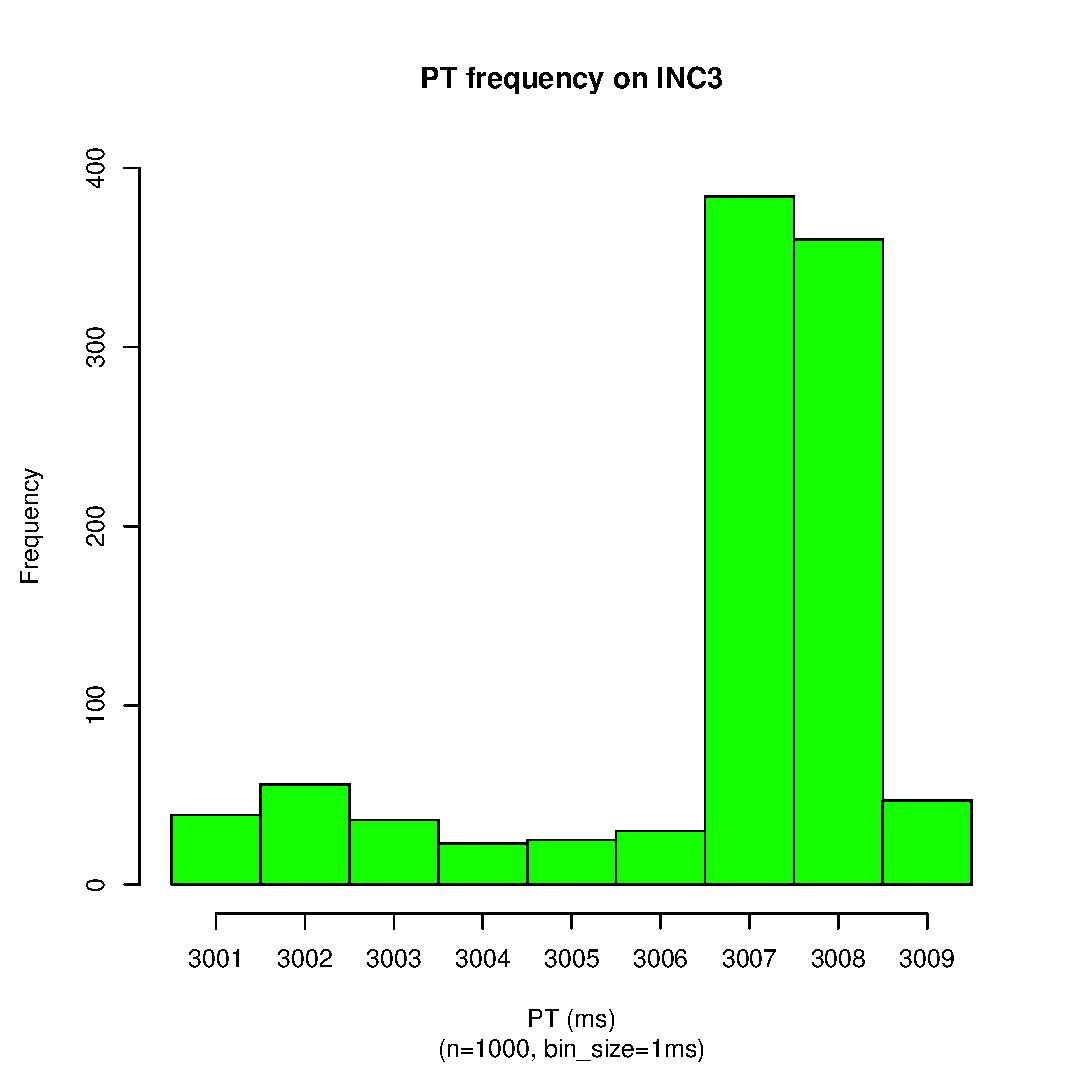
\includegraphics[scale=0.43]{u_s_time/3_sec_pt_hist.eps}
		\label{fig:inc3_pt_hist}
	}
	\subfigure[PT frequency on INC6 on {\tt sodb9}]{
		\includegraphics[scale=0.43]{u_s_time/6_sec_pt_hist.eps}
		\label{fig:inc6_pt_hist}
	}
	\subfigure[PT frequency on INC12  on {\tt sodb9}]{
		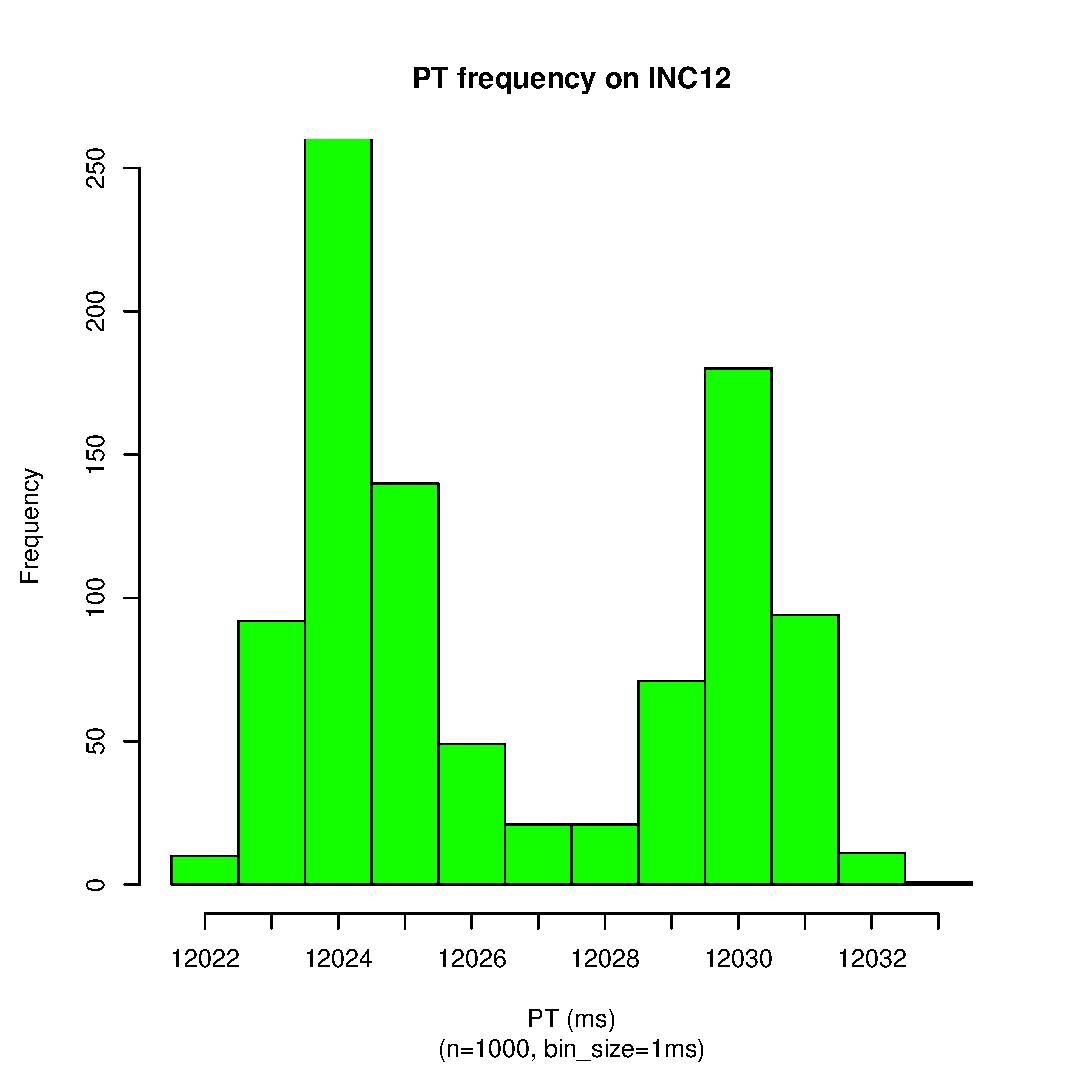
\includegraphics[scale=0.43]{u_s_time/12_sec_pt_hist.eps}
		\label{fig:inc12_pt_hist}
	}
	\subfigure[PT frequency on INC24 on {\tt sodb9}]{
		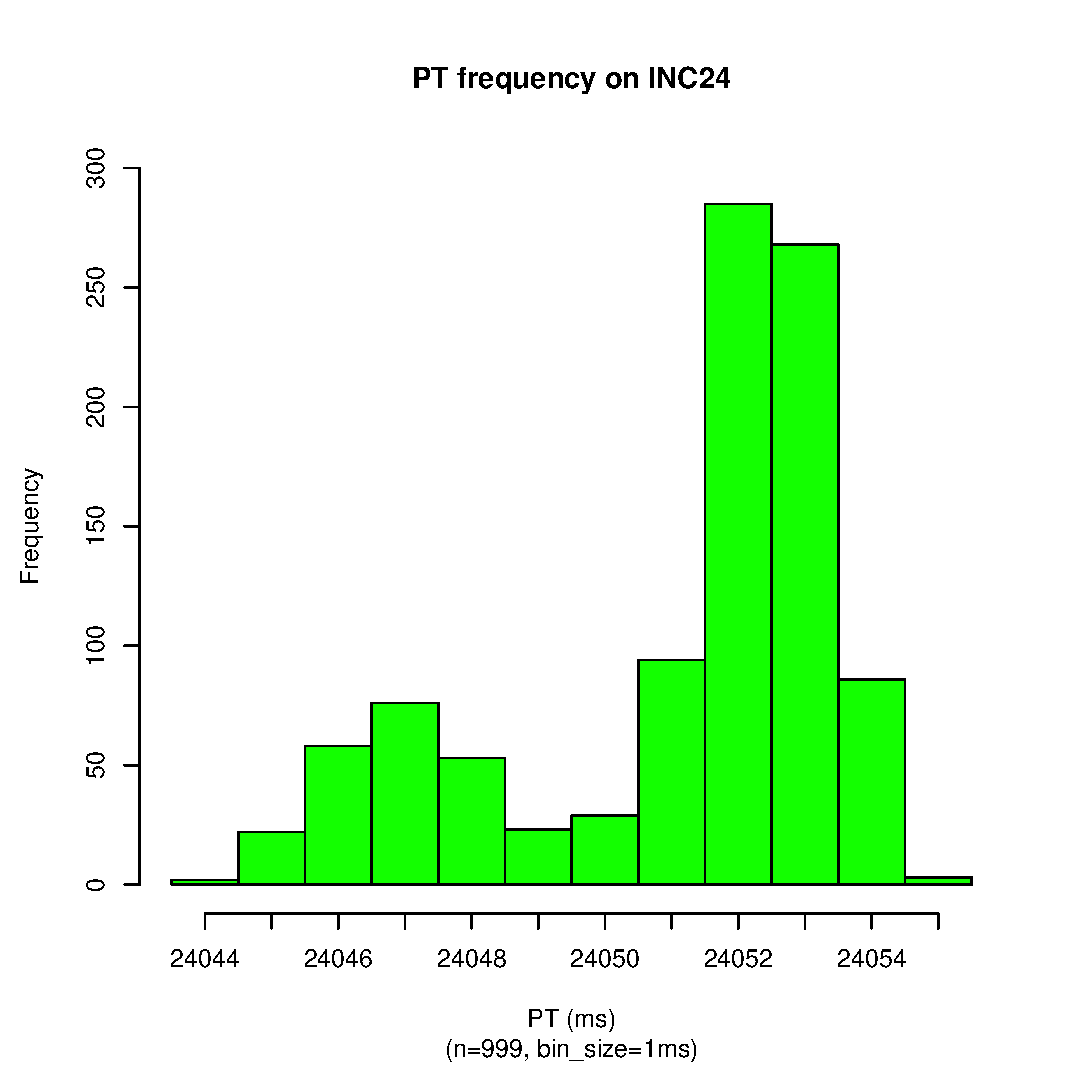
\includegraphics[scale=0.43]{u_s_time/24_sec_pt_hist.eps}
		\label{fig:inc24_pt_hist}
	}
	\caption{PT Histograms of INC3 ... INC24~\label{fig:new_pt_hist1}}
\end{figure}

\pagebreak
\newpage

\begin{figure}[hp!]
	\centering
	\subfigure[PT frequency on INC48 on {\tt sodb9}]{
		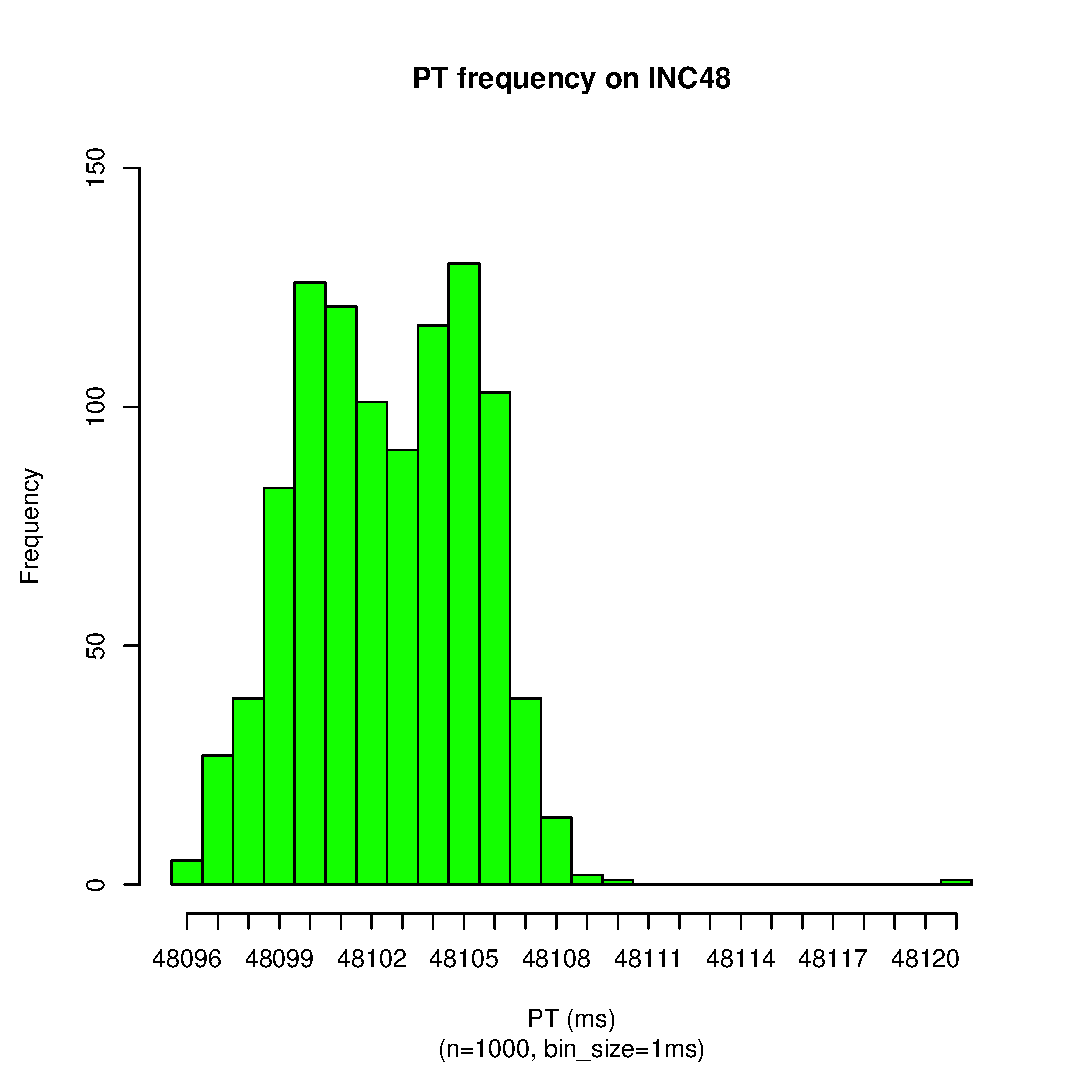
\includegraphics[scale=0.43]{u_s_time/48_sec_pt_hist.eps}
		\label{fig:inc48_pt_hist}
	}
	\subfigure[PT frequency on INC72 on {\tt sodb9}]{
		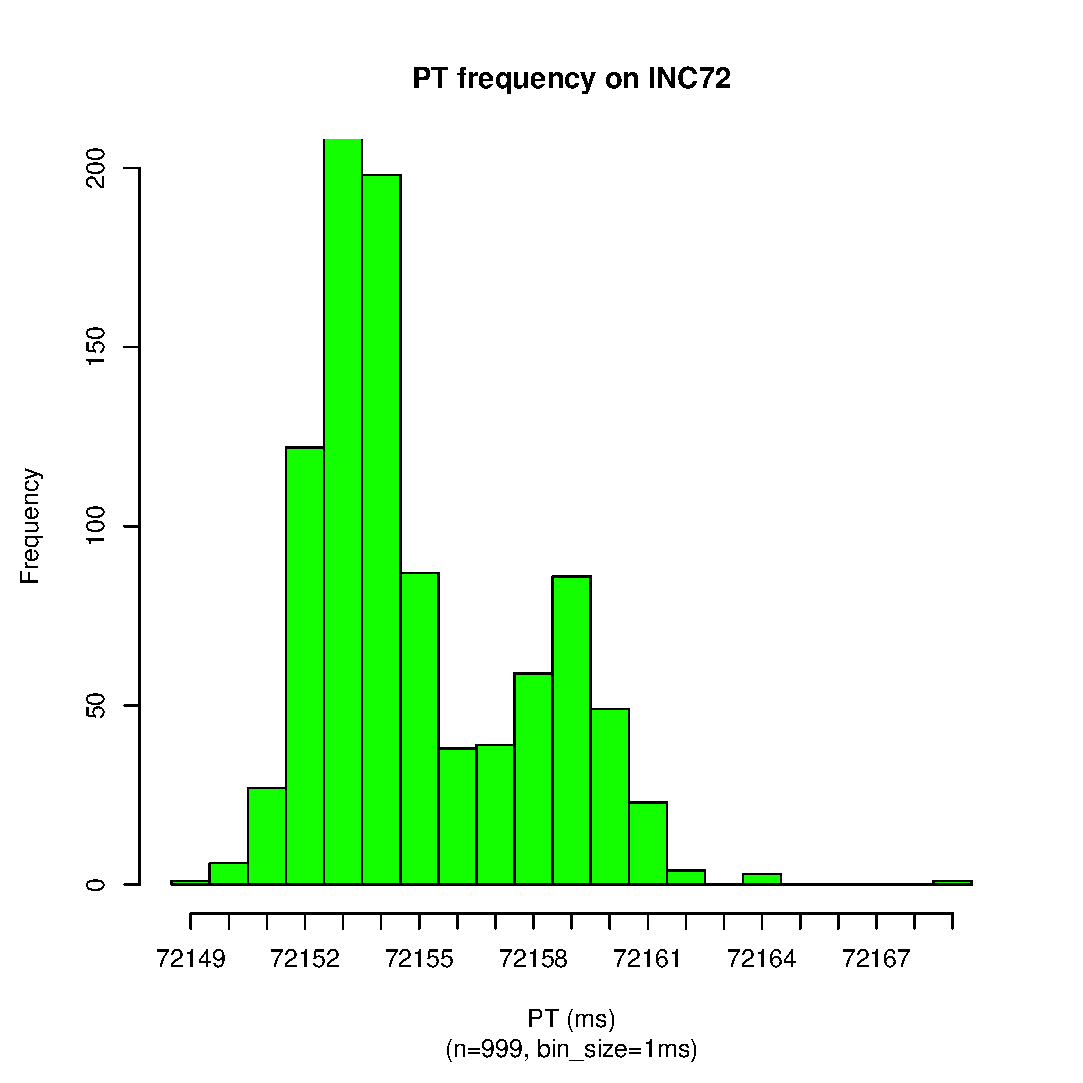
\includegraphics[scale=0.43]{u_s_time/72_sec_pt_hist.eps}
		\label{fig:inc72_pt_hist}
	}
	\subfigure[PT frequency on INC80 on {\tt sodb9}]{
		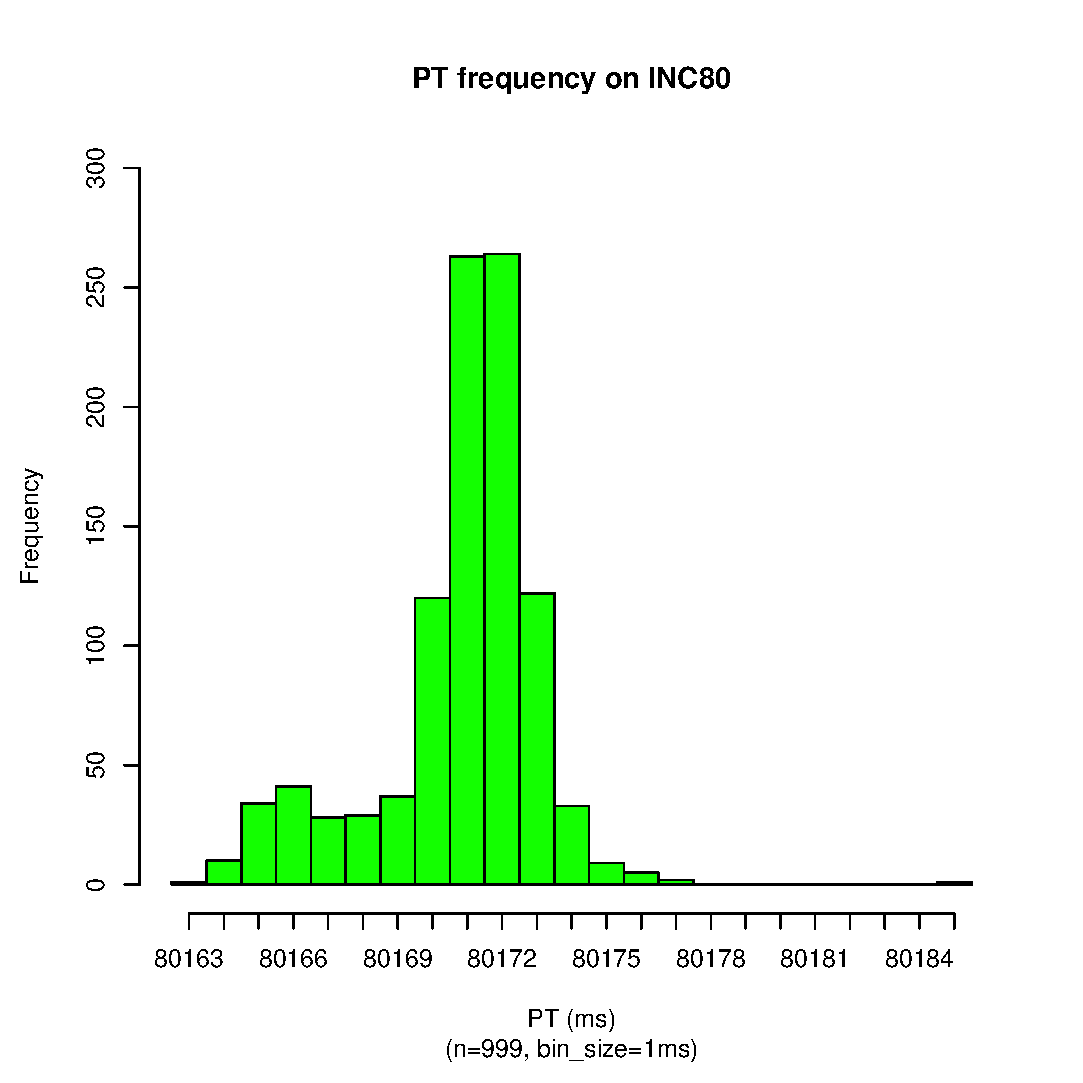
\includegraphics[scale=0.43]{u_s_time/80_sec_pt_hist.eps}
		\label{fig:inc80_pt_hist}
	}
	\subfigure[PT frequency on INC88 on {\tt sodb9}]{
		\includegraphics[scale=0.43]{u_s_time/88_sec_pt_hist.eps}
		\label{fig:inc88_pt_hist}
	}
	\caption{PT Histograms of INC48 ... INC88~\label{fig:new_pt_hist2}}
\end{figure}

\pagebreak
\newpage

\begin{figure}[hp!]
	\centering
	\subfigure[PT frequency on INC96 on {\tt sodb9}]{
		\includegraphics[scale=0.43]{u_s_time/96_sec_pt_hist.eps}
		\label{fig:inc96_pt_hist}
	}
	\subfigure[PT frequency on INC104 on {\tt sodb9}]{
		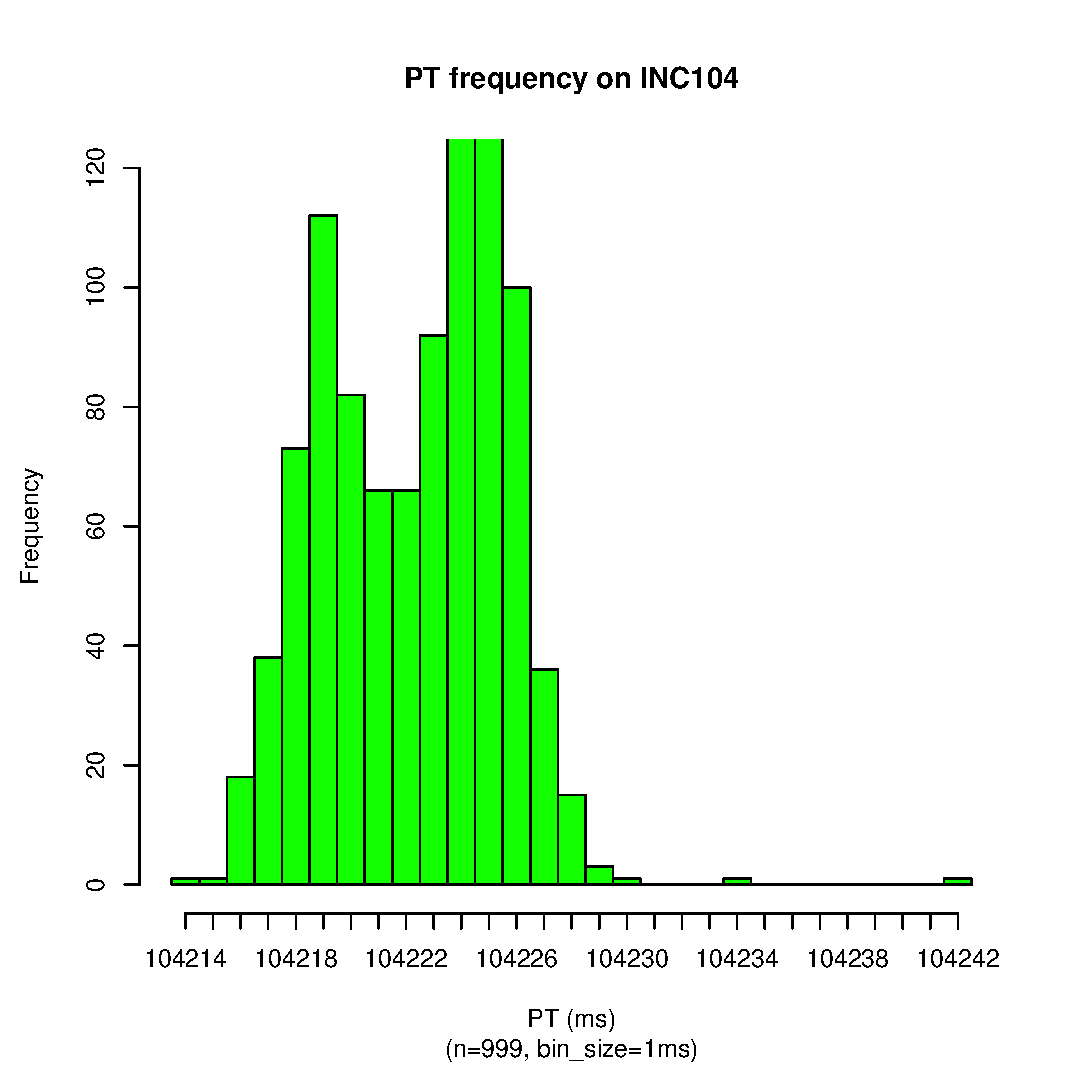
\includegraphics[scale=0.43]{u_s_time/104_sec_pt_hist.eps}
		\label{fig:inc104_pt_hist}
	}
	\subfigure[PT frequency on INC112 on {\tt sodb9}]{
		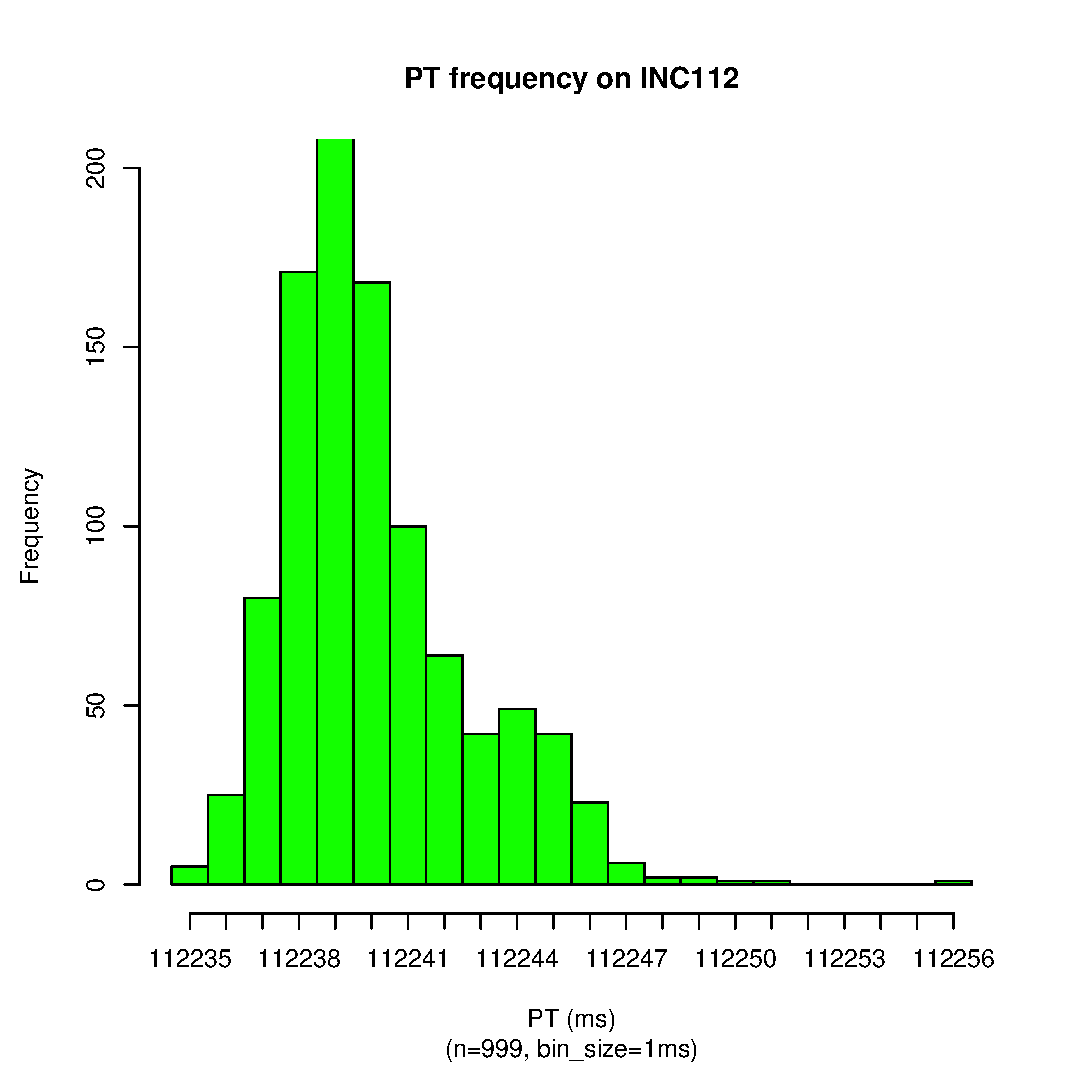
\includegraphics[scale=0.43]{u_s_time/112_sec_pt_hist.eps}
		\label{fig:inc112_pt_hist}
	}
	\subfigure[PT frequency on INC120 on {\tt sodb9}]{
		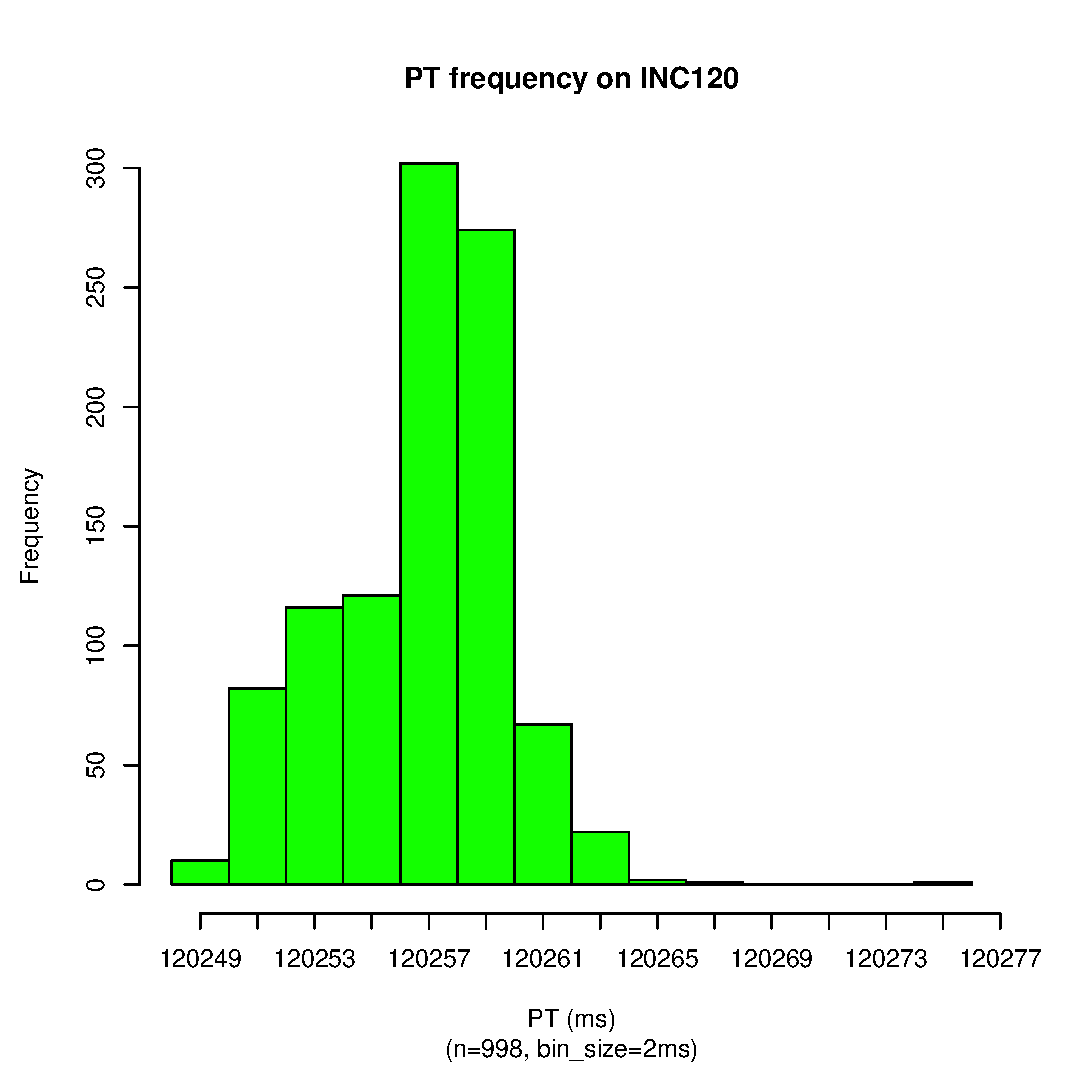
\includegraphics[scale=0.43]{u_s_time/120_sec_pt_hist.eps}
		\label{fig:inc120_pt_hist}
	}
	\caption{PT Histograms of INC96 ... INC120~\label{fig:new_pt_hist3}}
\end{figure}

\pagebreak
\newpage

\begin{figure}[hp!]
	\centering
	\subfigure[PT frequency on INC160 on {\tt sodb9}]{
		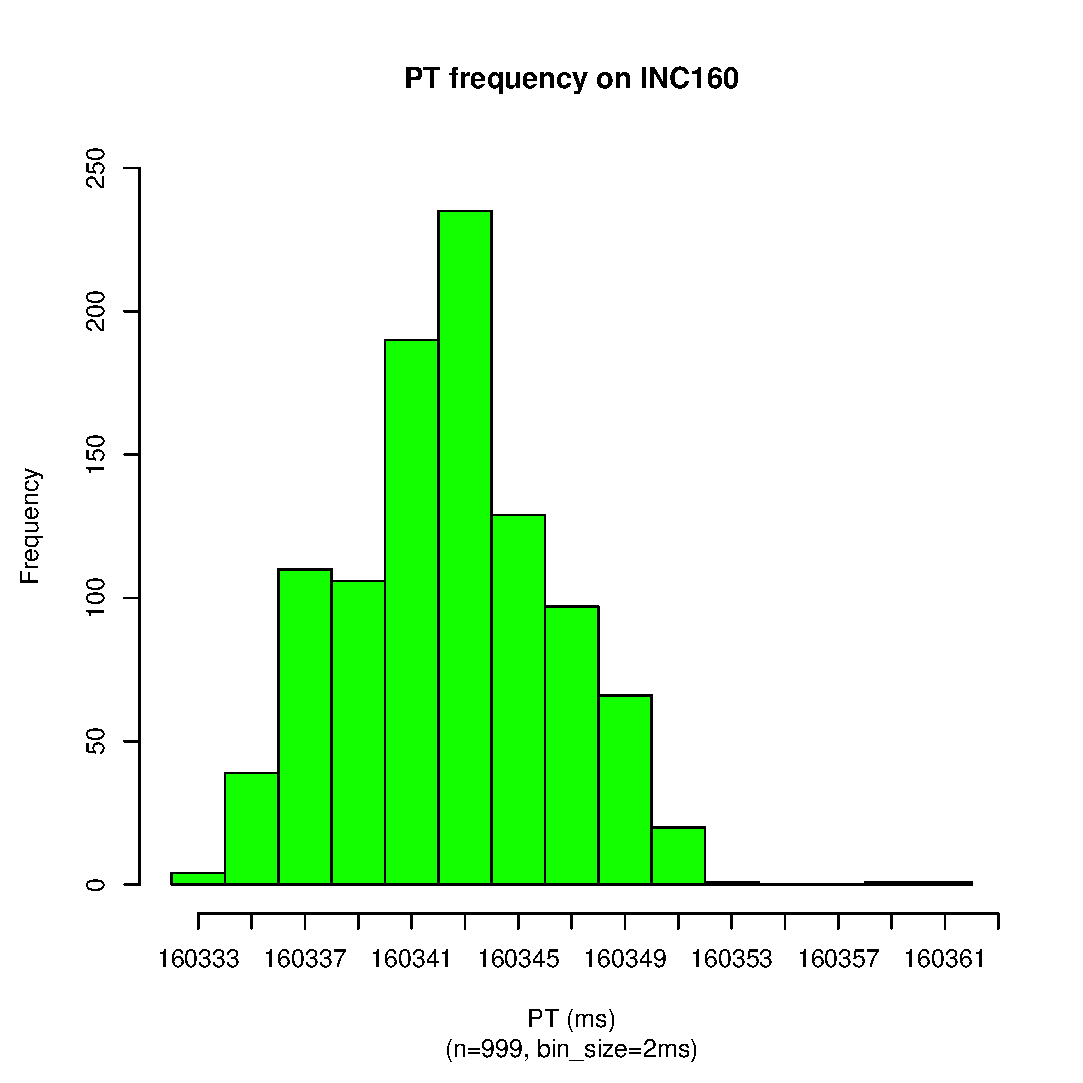
\includegraphics[scale=0.43]{u_s_time/160_sec_pt_hist.eps}
		\label{fig:inc160_pt_hist}
	}
	\subfigure[PT frequency on INC192 on {\tt sodb9}]{
		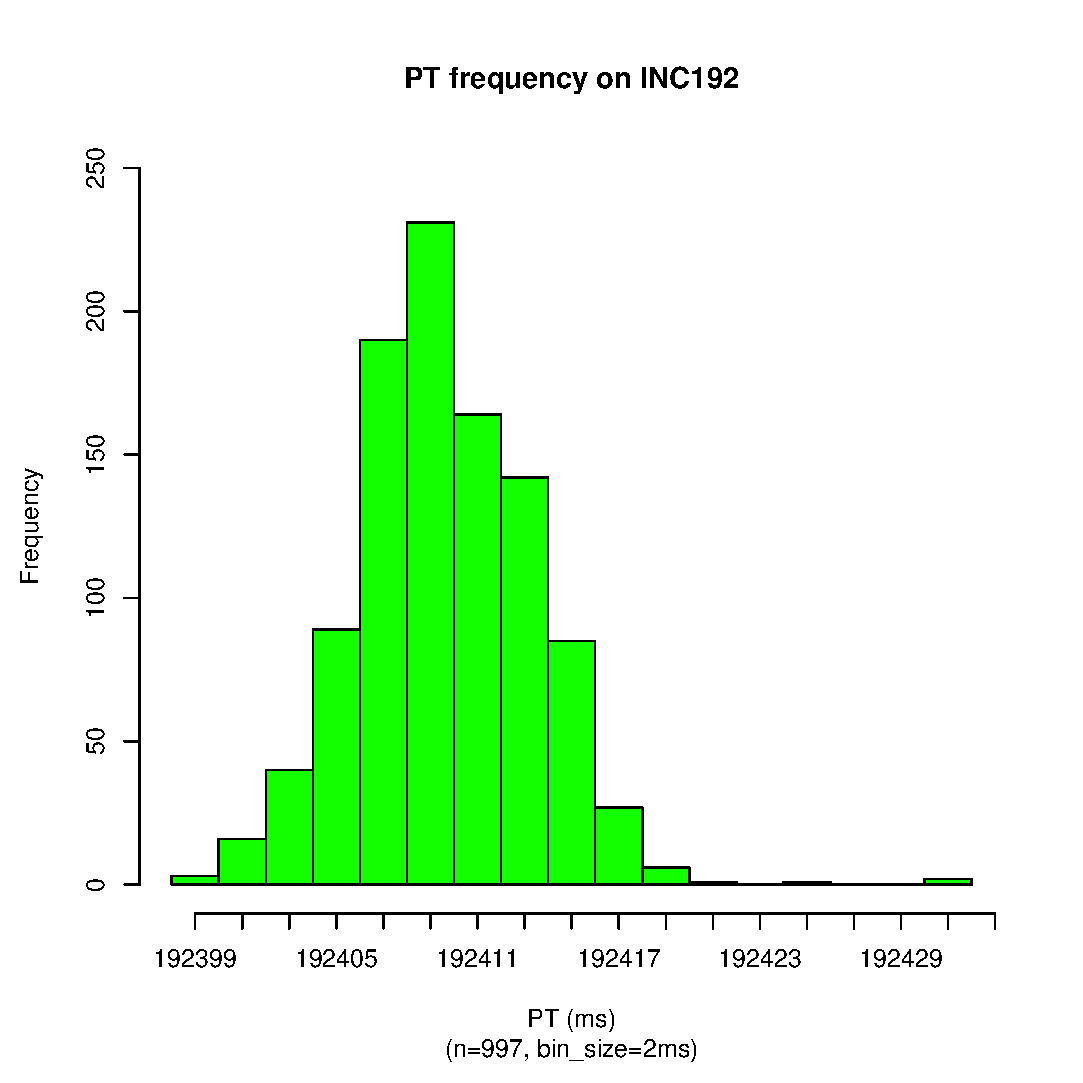
\includegraphics[scale=0.43]{u_s_time/192_sec_pt_hist.eps}
		\label{fig:inc192_pt_hist}
	}
	\subfigure[PT frequency on INC224 on {\tt sodb9}]{
		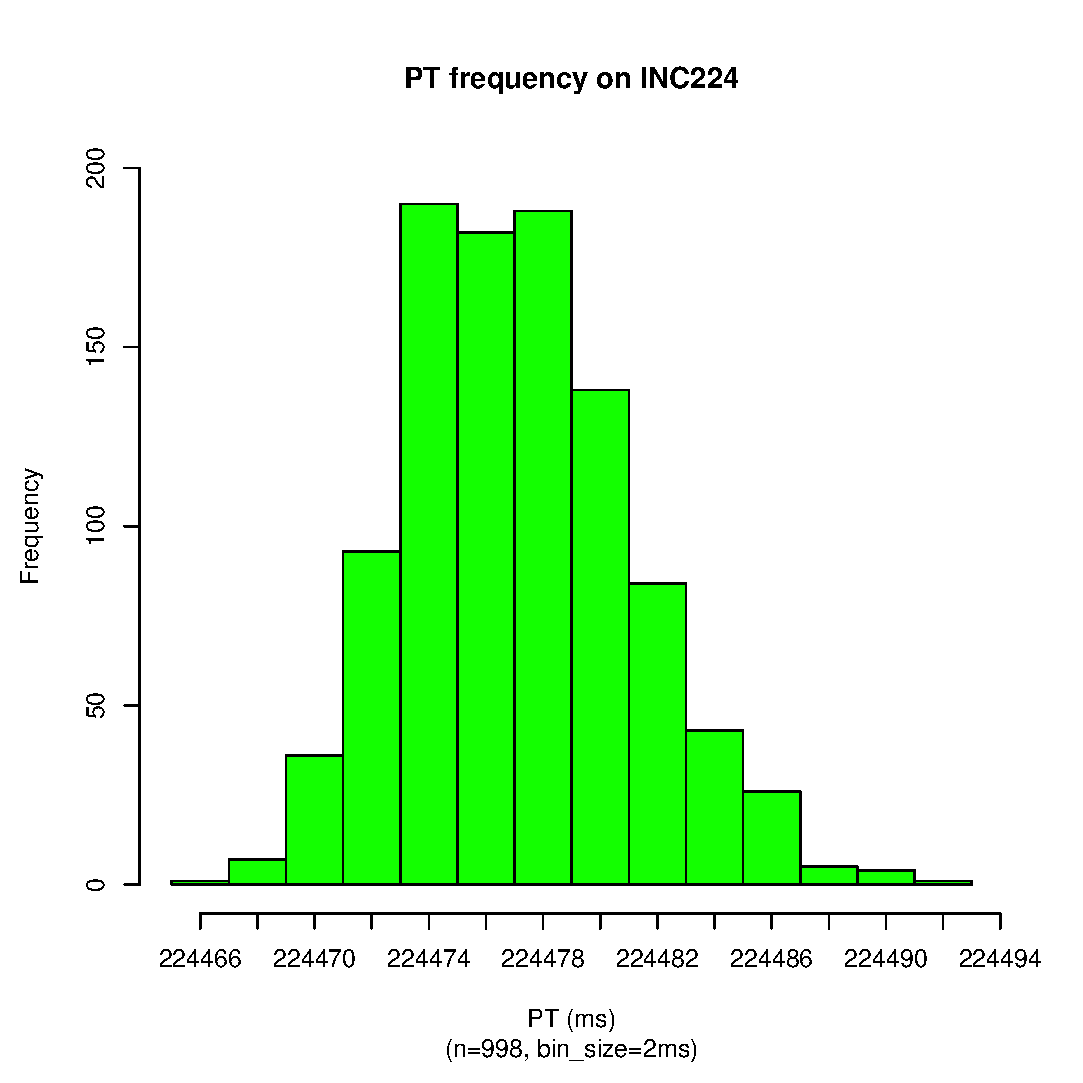
\includegraphics[scale=0.43]{u_s_time/224_sec_pt_hist.eps}
		\label{fig:inc224_pt_hist}
	}
	\caption{PT Histograms of INC169 ... INC224~\label{fig:new_pt_hist4}}
\end{figure}

\pagebreak
\newpage

\subsection{Summary}

\paragraph{Stacked Histograms in a 3D Plot:}
Figure~\ref{fig:hist3d} represents a 3D plot of collecting the histograms of PT in Section~\ref{sec:1st_pt}. 
Note that we additionally include the histograms from the task lengths of 8192 and 16384 seconds, which will be shown in Figures~\ref{fig:inc8192_r2_hist_v5} and~\ref{fig:inc16384_r2_hist_v5} (on page~47). See the legend in the right hand side of the figure, for more details about specific task length information. 
(To obtain the better shape, we could remove from those histograms the outliers that are identified via the second step of EMPv5.)
The x-axis corresponds to the normalized PT relative to the minimum, ranging 0 to 100, the y-axis to task length in log scale, and the z-axis to the normalized frequency relative to the highest bar for each histogram.

One thing to notice is that there are some runs having a few empty bins 
in their respective histogram. For instance, INC32 has such an empty bin as shown in Figure~\ref{fig:inc32_r1_et_hist_v5}. 
Same with INC256 in Figure~\ref{fig:inc256_r1_et_hist_v5}. For such an INC run, the z-axis associated with its histogram has the zero value on the x-axis in Figure~\ref{fig:hist3d}. 

\begin{figure}[htp!]
%\vspace{-.3in}
	\centering
	%\includegraphics[scale=0.6,angle=270]{u_s_time/3d_plot.eps}\label{fig:3d_plot}
	%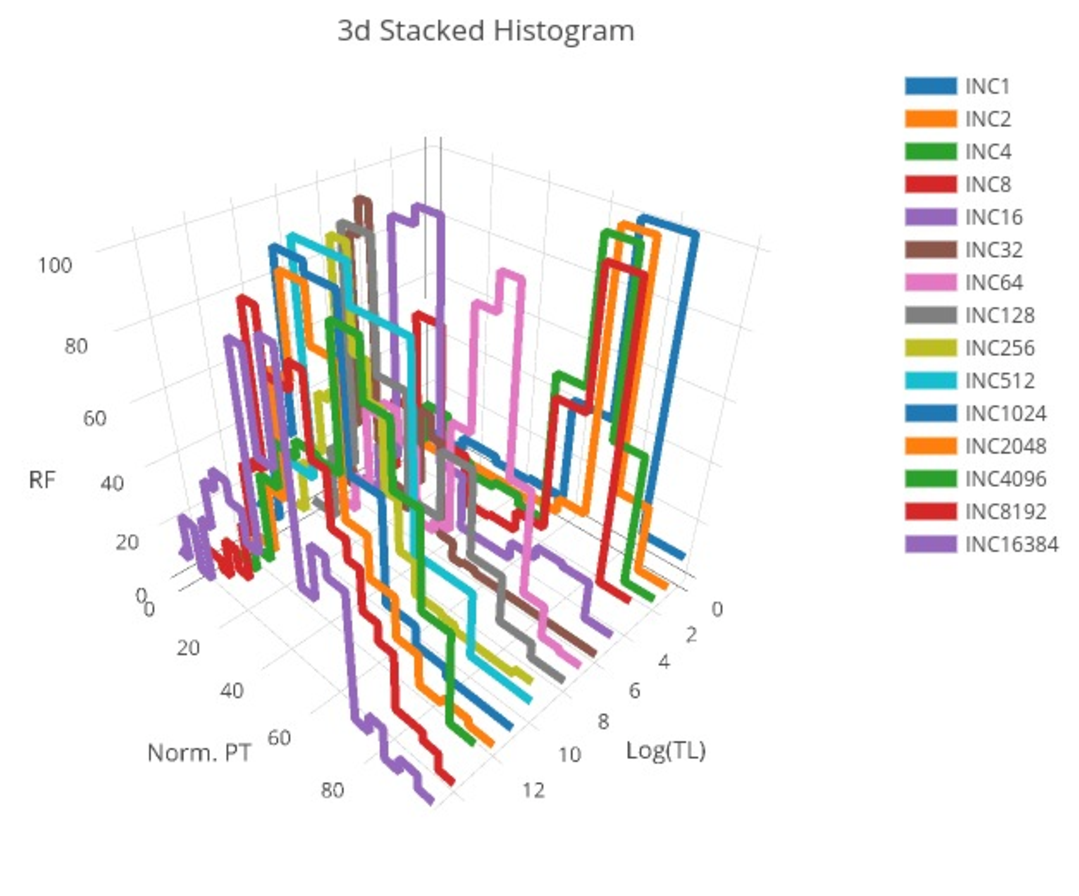
\includegraphics[scale=0.6]{u_s_time/new_3d_plot}\label{fig:3d_plot}
	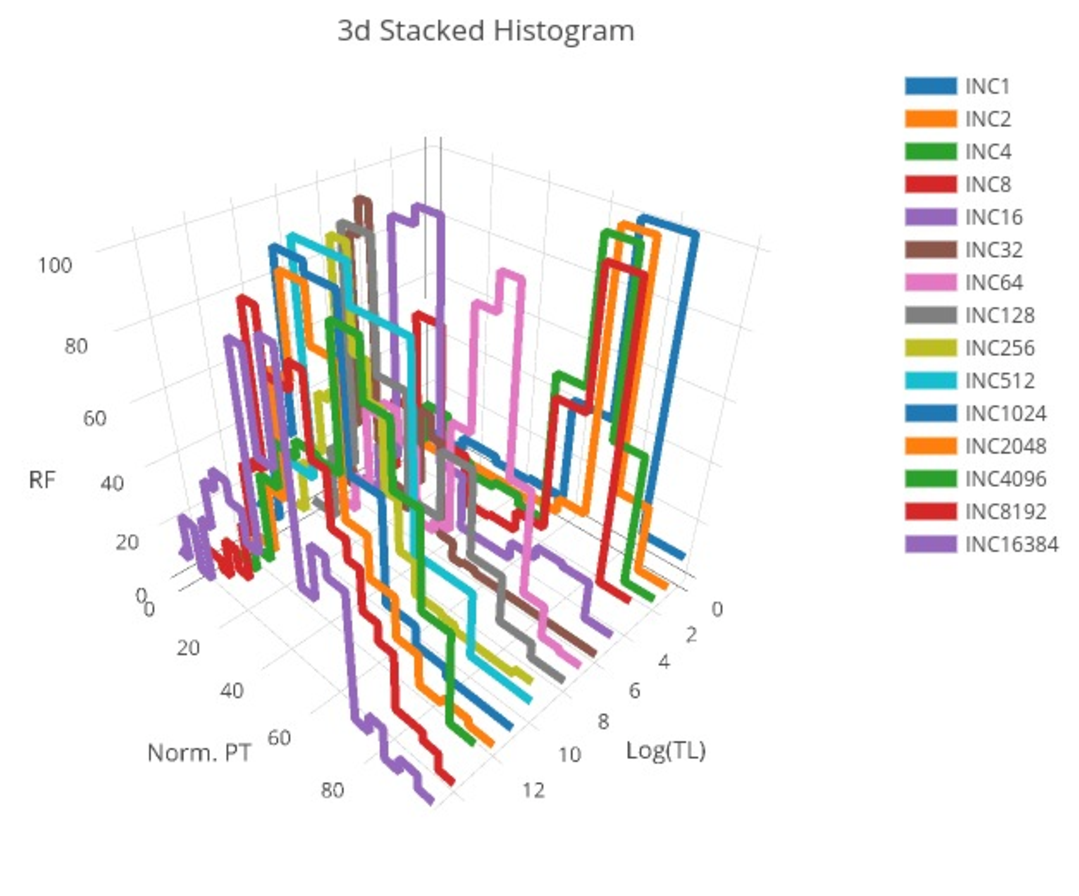
\includegraphics[scale=1]{u_s_time/new_3d_plot}\label{fig:3d_plot}
	\caption{3D histograms of PT on doubly-increasing INC on {\tt sodb9} for up to INC1024, on {\tt sodb10} for INC2048, on {\tt sodb12} for INC4096~\label{fig:hist3d}}
\end{figure}

\pagebreak
\clearpage
Figure~\ref{fig:hist3d_u} represents a 3D plot of collecting the histograms of user time only
exhibited in Section~\ref{sec:first_run}. 
\begin{figure}[htp!]
%\vspace{-.3in}
	\centering
	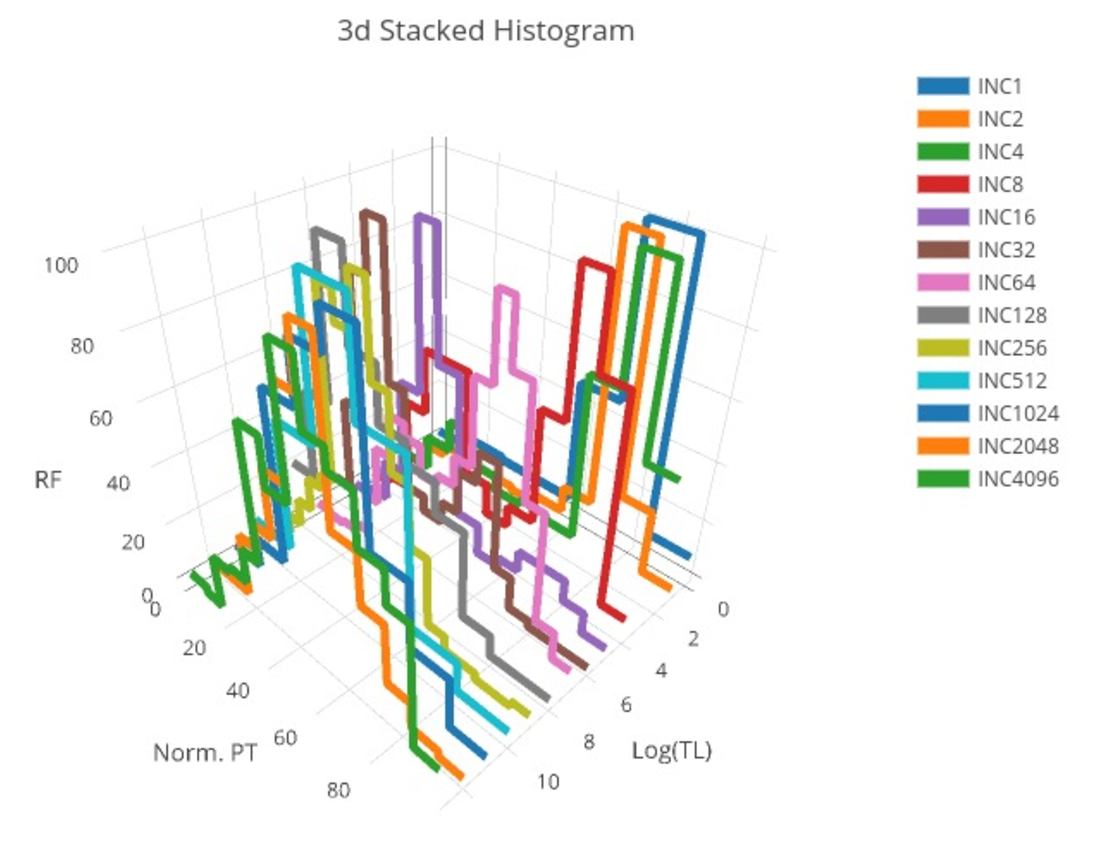
\includegraphics[scale=1]{u_s_time/3dplot_utime_only}\label{fig:3d_plot_u}
	\caption{3D histograms on INC on {\tt sodb9} for up to INC1024, on {\tt sodb10} for INC2048, on {\tt sodb12} for INC4096: user time only~\label{fig:hist3d_u}}
\end{figure}

\clearpage
\pagebreak

\paragraph{Fitting PT Histograms in Bi-Normal Distributions:}
We ran Rob's code to obtain a bi-normal fit for each INC's PT histogram 
in Section~\ref{sec:first_run}. 
Table~\ref{tab:binormal_fit} exhibits the total range of bins, the two means (modes), standard deviations, scales (weights) 
for the PT histogram, and figure numbers associated with each INC.

\begin{table}[h]
\begin{center}
\begin{tabular}{|l|l|l|l|l|l|l|l|l|} \hline
INC        & Total Range & Mean 1 & Mean 2 & Std 1 & Std 2 & Scale 1 & Scale 2 & Figures \\ \hline
INC1      & 6 & 1.66  & 4.73 & 1.03 & 0.54 & 0.10 & 0.90  & Fig.~\ref{fig:inc1_r1_hist_v5}\\ \hline
INC2      & 9 & 2.33  & 7.07 & 2.38 & 0.54 & 0.16 & 0.84  & Fig.~\ref{fig:inc2_r1_hist_v5} \\ \hline
INC4      & 9 & 2.17  & 7.89 & 0.99 & 0.86 & 0.21 & 0.79  & Fig.~\ref{fig:inc4_r1_hist_v5} \\ \hline
INC8      & 9 & 3.51  & 9.15 & 1.10 & 1.08 & 0.39 & 0.61  & Fig.~\ref{fig:inc8_r1_hist_v5}\\ \hline
INC16    & 10 & 4.04  & 9.53 & 0.98 & 1.28 & 0.83 & 0.17  & Fig.~\ref{fig:inc16_r1_hist_v5}\\ \hline
INC32    & 22 & 2.76  & 8.26 & 1.28 & 1.12 & 0.73 & 0.27  & Fig.~\ref{fig:inc32_r1_hist_v5}\\ \hline
INC64    & 14 & 6.36  & 12.02 & 1.64 & 1.62 &  0.35 & 0.65  & Fig.~\ref{fig:inc64_r1_hist_v5}\\ \hline
INC128  & 16 & 4.21  & 8.64 & 1.82 & 3.40 & 0.41 & 0.59  & Fig.~\ref{fig:inc128_r1_hist_v5}\\ \hline
INC256  & 38 & 6.08  & 14.61  & 3.59 & 3.75 & 0.12 & 0.88  & Fig.~\ref{fig:inc256_r1_hist_v5}\\ \hline
INC512  & 20 & 1.60  & 12.43   & 11.51 & 4.47 & 0.08 & 0.92  & Fig.~\ref{fig:inc512_r1_hist_v5}\\ \hline
INC1024 & 40 & 1.13  & 18.88  & 14.99 & 6.01 & 0.06 & 0.94 & Fig.~\ref{fig:inc1024_r1_hist_v5}\\ \hline
INC2048 & 65 & 29.93 & 52.92 & 8.53 & 6.59 & 1.00 & -0.00 & Fig.~\ref{fig:inc2048_r1_hist_v5}\\ \hline
INC4096 & 65 & 39.57 & 98.00 & 12.41 & 8.19 & 0.94 & 0.06  & Fig.~\ref{fig:inc4096_r1_hist_v5}\\ \hline
\end{tabular}
\end{center}
\vspace{-.2in}
\caption{Two means in mode computed for each INC~\label{tab:binormal_fit}}
\end{table}

\pagebreak
\clearpage

\begin{figure}[htp!]
	\centering
	\subfigure[Mean]{
		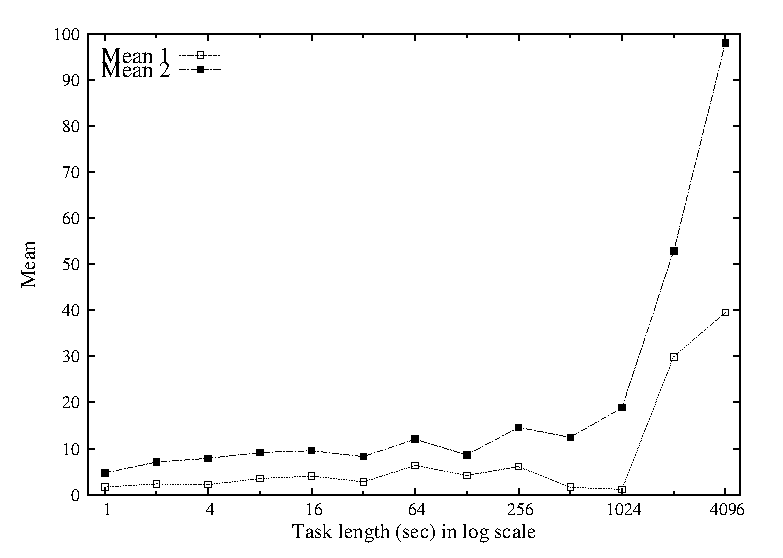
\includegraphics[scale=0.6]{u_s_time/binormal_fit_mean.eps}
		\label{fig:binormal_mean}
	}
	\subfigure[Standard Deviation]{
		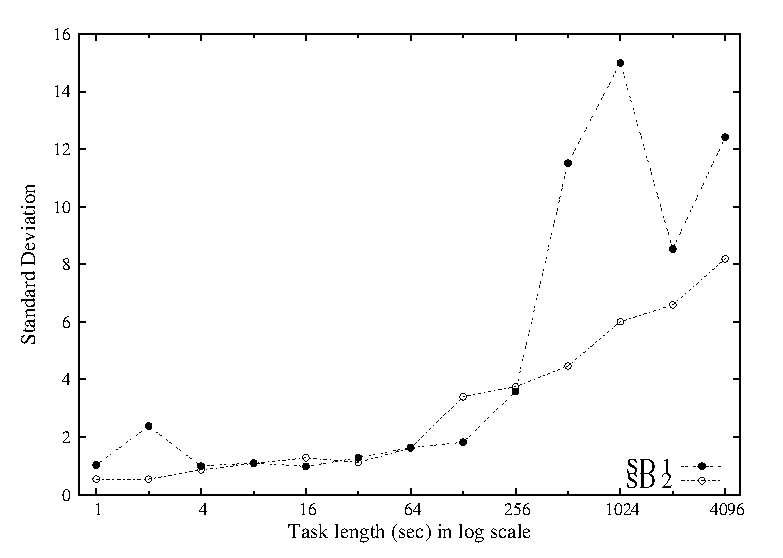
\includegraphics[scale=0.6]{u_s_time/binormal_fit_std.eps}
		\label{fig:binormal_std}
	}
	\subfigure[Scale]{
		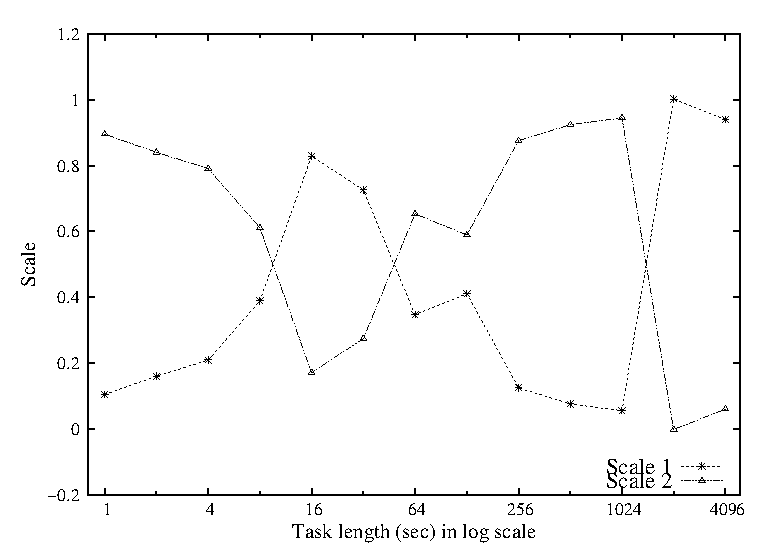
\includegraphics[scale=0.6]{u_s_time/binormal_fit_scale.eps}
		\label{fig:binormal_scale}
	}
	\caption{Plots of two means, standard deviations, and scales for each INC 
	over increasing task length: based on Table~\ref{tab:binormal_fit}\label{fig:bnormal_Fit}}
\end{figure}

\clearpage
\pagebreak

%\subsection{Absolute and Relative Variance over Increasing Task Lengths}
\paragraph{Absolute and Relative Variance over Increasing Task Lengths:}
Figure~\ref{fig:cv_inc} exhibits absolute and relative variances over increasing task lengths. 
More specifically, Figures~\ref{fig:overall_std} and~\ref{fig:overall_std_log} 
concern the PT standard deviations of all the runs including those two longest runs of INC8192 and INC16384 described in Table~\ref{tab:exp_notes2}. 
The x-axis is task length, and the y-axis standard deviation; Figure~\ref{fig:overall_std_log} is taken in log scale.
Figures~\ref{fig:overall_re} and~\ref{fig:overall_re2} shows 
the relative variance of the same data set---{\em coefficient of variation} (= standard deviation 
/ task length (or mean)). Both of the x and y axes in these two figures are taken in log scale. 
We also overlap a linear-square-fit of each case on the same figure. 

\begin{figure}[htp!]
	\centering
	\subfigure[Standard deviation (absolute)]{
		%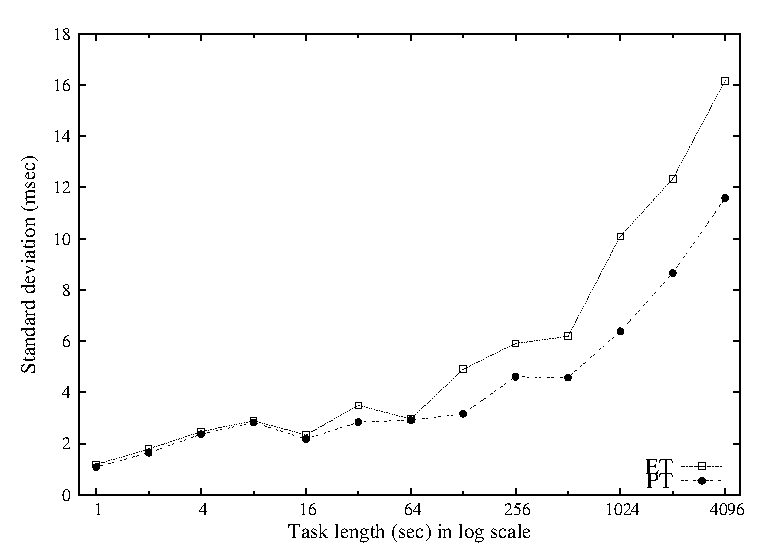
\includegraphics[scale=0.6]{u_s_time/overall_std.eps}
		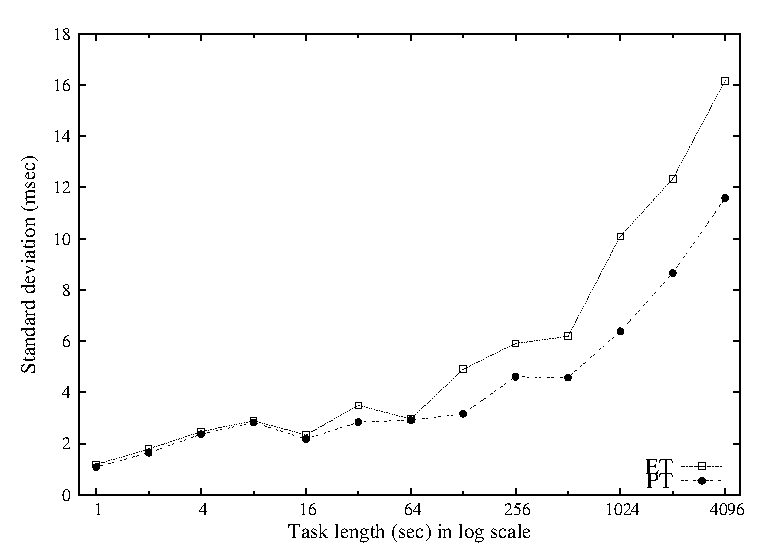
\includegraphics[scale=0.6]{u_s_time/new_overall_pt_std.eps}
		\label{fig:overall_std}
	}
	\subfigure[Standard deviation (absolute) in log scale]{
		%\includegraphics[scale=0.6]{u_s_time/overall_std_log.eps}
		\includegraphics[scale=0.6]{u_s_time/new_overall_pt_std_log.eps}
		\label{fig:overall_std_log}
	}
	\subfigure[Coefficient of variation in log scale (relative): divisor=mean]{
		\includegraphics[scale=0.6]{u_s_time/overall_pt_re.eps}
		\label{fig:overall_re}
	}
	\subfigure[Coefficient of variation in log scale (relative): divisor=task length]{
		\includegraphics[scale=0.6]{u_s_time/new_overall_pt_re.eps}
		\label{fig:overall_re2}
	}
	\caption{Absolute and relative variances~\label{fig:cv_inc}}
\end{figure}

